\chapter{Analysing DRL Agents Trained with Domain Randomisation}
\label{ch:drl_interp}
\section{Introduction}
% In previous chapters, we have discussed several methods to improve sample efficiency in deep reinforcement learning (DRL), especially in complex robot manipulation tasks with continuous, rather than discrete, control. 
In this thesis, we first provide a comprehensive analysis on the trained DRL agents, which aims to understand features and policies that the agents learned in the environment. Specifically, proximal policy optimisation (PPO)~\cite{schulman2017proximal} is selected as the DRL algorithm to train the model, because it is widely used in a variety of scenarios~\cite{berner2019dota,rajeswaran2017learning,vinyals2019grandmaster}, we believe that this analysis can provide more insight to the community. In the following chapters, we will further improve the sample efficiency of PPO algorithm with different ways in the tasks with sparse or delayed rewards. Recently, most DRL experiments are performed in a simulated environment. Training becomes much more problematic when applying DRL to real-world applications. For example, in a robot manipulation task, which requires an agent to pick up a cube and place it in a target position, computer vision techniques, such as object detection, pose estimation, or semantic segmentation, are used to estimate the position and orientation of the cube. Then, at each timestep, the current information of the cube and the proprioceptive data of the robot arm are provided to the RL agent to select an action. 

%To reduce \td{real-world training times}, 
A number of end-to-end approaches~\cite{gu2017deep,levine2016end,zhu2017target} have been proposed in recent years, which enable the agent to infer the policy according to raw observations (e.g., images) directly. However, such an end-to-end training setup would require the agent to collect samples for a long time in a real-world environment to update the policy network, which may increase the risk of robot/hardware failure and thus elevate the cost of training significantly. An emerging solution is to have the agent trained in a simulated environment before transferring the policy to the real world. In this period, the agent also needs to overcome the ``reality gap"~\cite{jakobi1995noise} between the simulated environment and the real-world environment, and domain randomisation (DR)~\cite{andrychowicz2018learning,james2017transferring,peng2018sim,sadeghi2017cad2rl,tobin2017domain} is a widely used approach for this purpose. When using DR in training, the elements of the simulated environment are varied to some extent, from the visual appearance to the environment dynamics (see Figure~\ref{fig:dr_example}), in order to improve the policy's robustness to various changes in the environment.
\begin{figure}[h!]
  \centering
  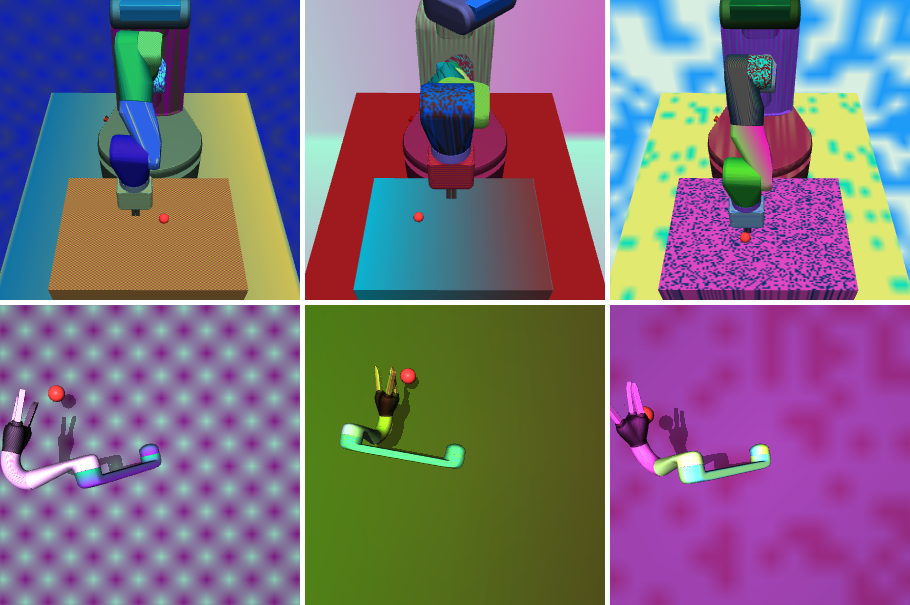
\includegraphics[width=\linewidth]{figures/chapter6/domain_random.png}
  \caption[Examples of visual domain randomisation in the simulated robot environments.]{Examples of domain randomisation (visual appearances) in the simulated Fetch (top) and Jaco (bottom) robots environments.}
  \label{fig:dr_example}
\end{figure}

However, such an end-to-end training paradigm, which could involve inferring actions based on image inputs, makes the theoretical analysis of both the environment and the agents that act within it practically infeasible. Specifically, deep neural networks (NNs) trained with DRL form a direct ``black box" mapping from observation to action, presenting the challenge of understanding learned control strategies. If we would like to deploy such policies---particularly on robots in the real world---we would also want to be able to \emph{explain} them~\cite{arrieta2020explainable}. An interpretation of the inference of a model can be used not only as a way of explaining the behaviour of the model, but can also be used to characterise other properties, such as safety, fairness, and reliability ~\cite{doshi2017towards}. Although there are many existing approaches to explain NNs~\cite{guidotti2018survey}, each of these methods is subjective to varying degrees.
\begin{figure}[h!]
  \centering
  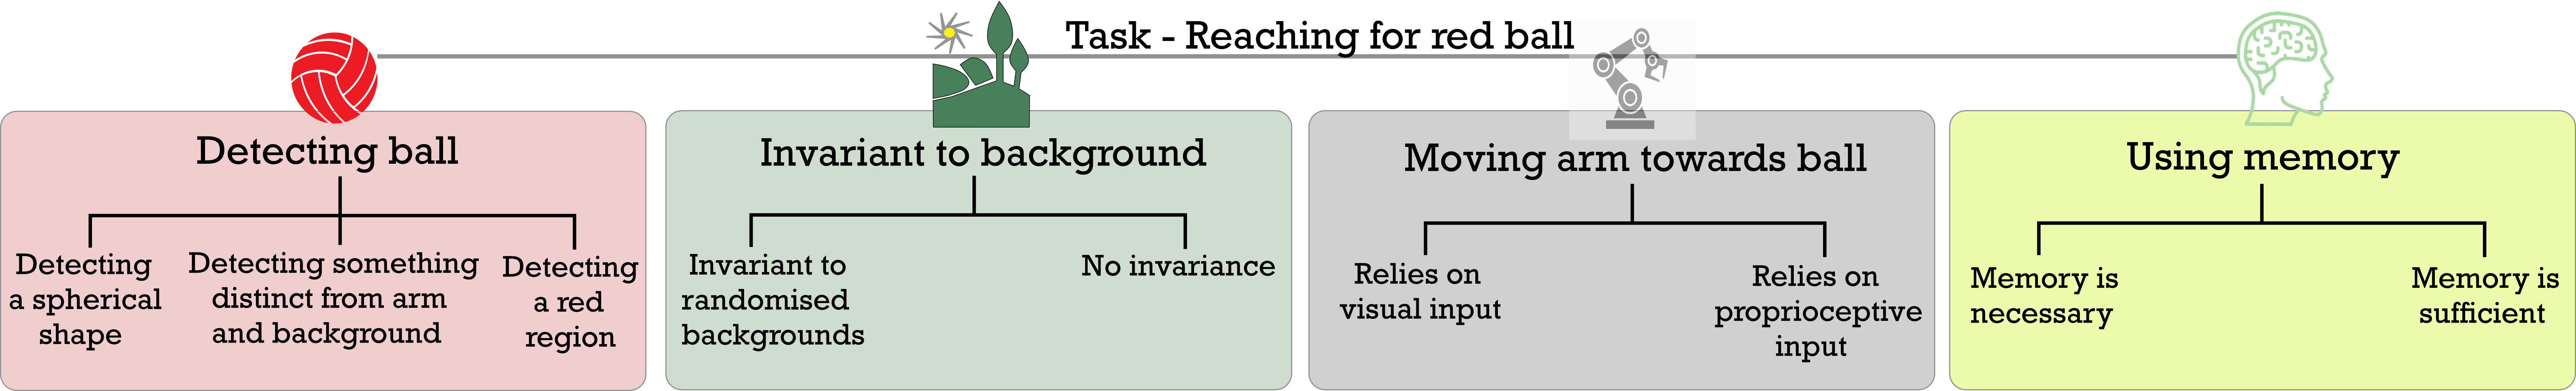
\includegraphics[width=\linewidth]{figures/chapter6/strategies.png}
  \caption[The range of strategies an agent may learn to use when trained to reach a red target.]{The range of strategies an agent may learn to use when trained to reach a red target, which we split into three components. Firstly, the agent must visually localise the target---which can be accomplished by detecting red, spherical objects, or simply anything with a significant red component. Secondly, the agent can use vision and/or proprioception to guide its arm to the target. Finally, the agent may accomplish the task with varying levels of robustness to changes in the rest of the visual scene. Using a range of analyses, we show that agents trained to accomplish the same task learn different subsets of these strategies, depending on their training conditions. [This diagram was created by Dr.Kai Arulkumaran and Tamara Gerbert~\cite{dai2022analysing}.]}
  \label{fig:strategies}
\end{figure}

In this chapter, we aim to understand how DRL agents make decision in the environment and understand how agents trained with visual DR behave differently from agents trained without. To this end, we train DRL agents under a range of different settings and use relative differences to better interpret their policies. In contrast to most prior work examining DRL policies~\cite{atrey2020exploratory,greydanus2018visualizing, olson2021counterfactual,puri2020explain,rupprecht2020finding,such2018atari,zahavy2016graying}, we not only provide explanations for how policies react to parts of states/individual states, but use our array of experiments to characterise their \emph{global} strategies (see Figure~\ref{fig:strategies}). Through these experiments and analysis, we are able to provide some insight into the following questions:
\begin{itemize}
    \item How robust are agents to unseen scenarios?
    \item To what extent are visual inputs rather than proprioceptive inputs used by the agent?
    \item How redundant is the network in its representation? 
    \item What is rate of learning in different layers under different training configurations?
\end{itemize}
%For instance, we examine the relative importance of different input modalities, and whether agents need their memory to complete tasks. 

In particular, we train different robots with vision-based inputs to perform the task of reaching for a (red) target, and then use different techniques to understand what features of the environment the policies react to. \textit{Unlike} many experiments reported in the literature~\cite{andrychowicz2017hindsight,fang2018dher,fang2019curriculum}, the agent does not have direct access to the coordinates of the ball as a state. Under certain training settings, the agent may localise the target by simply looking for anything red, and it is only under more challenging training conditions that the agent utilises both colour and shape. Clearly, the latter strategy better represents what we want a real-world agent to learn, while the former is merely a ``shortcut'' \cite{geirhos2020shortcut}.

The structure in this chapter is organised in a different way from the previous ones. In Section~\ref{ch6:sec_interp}, we first introduce the interpretability techniques used in this work. In Section~\ref{ch6:exp}, we detail our customised simulated environments, the network structure of DRL agents, training details, and the settings of test scenarios. Subsequently, in Section~\ref{ch6:results}, we conduct an exhaustive analysis on the trained models using a broad suite of interpretability techniques. Finally, in Section~\ref{ch6:discussion}, we discuss our findings and provide recommendations for applying interpretability techniques to DRL agents.

\section{Interpretability Techniques}
Neural networks (NNs) have achieved great success when used with reinforcement learning. However, compared to hand-crafted feature descriptors, NNs lack interpretability, and the networks are often treated as black boxes. Therefore, it is important that we are able to explain and understand what the NN has learned before deploying it in real-world applications, where safety and reliability are crucial. In this work, we focus on understanding the NN in a DRL training paradigm. To do so, various interpretability methods have been considered, which include saliency maps, unit ablations, layer re-initialisation and recurrent ablations. 
\label{ch6:sec_interp}
\subsection{Saliency Maps}
\begin{figure}[h!]
  \centering
  \begin{subfigure}{0.24\columnwidth}
    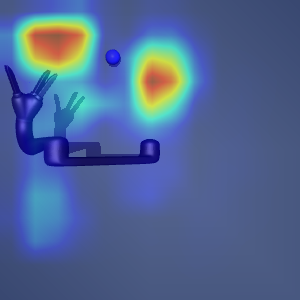
\includegraphics[width=\linewidth]{figures/chapter6/occ_jaco_baseline}
    \subcaption{Occ. (Gaussian)}
  \end{subfigure}
  \begin{subfigure}{0.24\columnwidth}
    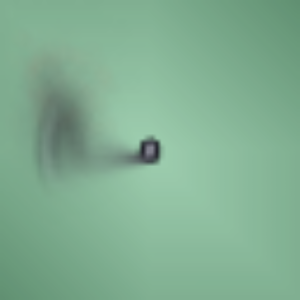
\includegraphics[width=\linewidth]{figures/chapter6/average_map_jaco_large.png}
    \subcaption{Avg. $\mathbf{x}^{base}$}
  \end{subfigure}
  \begin{subfigure}{0.24\columnwidth}
    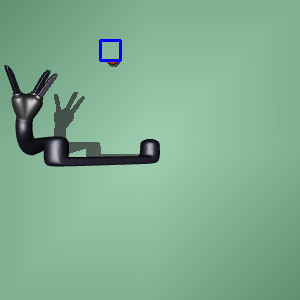
\includegraphics[width=\linewidth]{figures/chapter6/average_map_mask.png}
    \subcaption{Avg. $\mathbf{x}^{base}$ mask}
  \end{subfigure}
  \begin{subfigure}{0.24\columnwidth}
    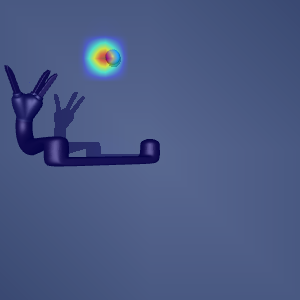
\includegraphics[width=\linewidth]{figures/chapter6/occ_jaco_average_map.png}
    \subcaption{Occ. (avg. $\mathbf{x}^{base}$)}
  \end{subfigure}
  \caption[Visualisation of different occlusion-based saliency map methods.]{Occlusion-based saliency map methods: (a) using Gaussian blur mask and (d) using an average image (b, c). Occlusion-based method using Gaussian blur masks (a) shows extra artifacts. Our improved saliency map method (d) highlights important regions in the result by using average baseline image created from plentiful trajectories (b). (c) shows one instance step that using the average baseline image as the occlusion in the original input. The occlusion region is highlighted with a blue outline.}
  \label{fig:saliency_baseline}
\end{figure}

Saliency maps are widely used to understand and explain the output of NNs. Similarly to previous work on understanding DRL agents~\cite{greydanus2018visualizing}, we also use an occlusion-based approach for interpreting. The occlusion-based method~\cite{zeiler2014visualizing} generally adopts a gray mask to scan the entire input image and then measures the variation of the output in each masked region to identify which areas have significant influences on the output of the NN. The variation of the performance is also called the saliency value, and it can be expressed as:
\begin{align}
S_{m, n} = \lVert F(\mathbf{x}) - F(\mathbf{x}_{m, n}^{occ}) \rVert_2,
\end{align}
where $(m, n)$ is the location on the image $\mathbf{x}$, $F(\mathbf{x})$ is the output of the original input, and $F(\mathbf{x}_{m, n}^{occ})$ is the output of the input with an occlusion mask at location $(m, n)$. In the work of~\cite{greydanus2018visualizing}, which aims to understand DRL agents in Atari games, the gray mask is replaced with a Gaussian blur mask. Because the agent only receives gray scale images in the training and testing. Thus, the gray mask can be recognised as a part of the gray object, and the Gaussian blur mask can introduce spatial uncertainty to find informative regions. 

However, the agent receives an RGB image as an input in our task. As a result, the occlusion-based method using Gaussian blur masks cannot highlight any important regions (see Figure~\ref{fig:saliency_baseline}a), and thus fails to provide any valuable information to understand the agent. Atrey \textit{et al.}~\cite{atrey2020exploratory} identify this issue of applying saliency methods to DRL agents as modifying observations in a manner that is incongruent with the true environment's state and generative process, and proposed intervening directly in the environment to employ counterfactual methods. However, in general, this level of control over the environment is not easy. In this work, we are more interested in task-specific objects in the environment, such as the robot arm and the red ball. To avoid interference from the occlusion-based masks on unimportant areas, we first sample 1,000 input frames with the trained policy from the environments (the policy is not updated during this process). Next, these 1000 frames are averaged to produce a baseline image (see Figure~\ref{fig:saliency_baseline}b). Then, we use this baseline image to generate the occlusion in the corresponding locations (see Figure~\ref{fig:saliency_baseline}c) in the input frame. Finally, we can measure the performance change and get an improved saliency map, which highlights the informative regions in the input image  (see Figure~\ref{fig:saliency_baseline}d).
%Inspired by the work which use reference images for the calculation of interpreta

Another recent study introduced a more robust DRL-specific saliency method~\cite{puri2020explain}, but it is only applicable to agents which learn a state-action value function over discrete action spaces.
%\subsection{Statistical and Structural Weight Characterisations}
\subsection{Channel-wise Unit Ablations}
Unit ablations evaluate the importance of a single unit in the convolutional layer by masking it to zero and examining the variations in the performance. In general, an important filter can lead to a significant performance drop. If a unit is set to zero and it has no effect on the ability to achieve a task, then it means one of two things: either the unit is redundant and performs no useful function in the network, or the function of the network is well-distributed amongst multiple neurons. While more sophisticated unit ablations have been applied in DRL~\cite{meyes2020you}, {this has only been in the context of a control task with a low-dimensional symbolic state space}. We further provide a Python style code snippet below to demonstrate the process of unit ablations.
\begin{minted}[frame=lines, mathescape, linenos]{python}
# Python code of unit ablations
import torch
for i in range(N_c): # N_c is the number of output channels
    net.load_state_dict(torch.load(ckpt_path))
    net.conv1.weight[i, :, :, :] = 0
    net.conv1.bias[i] = 0
    success_rate = eval(net)
\end{minted}
% Layer initialisation
\subsection{Layer Re-initialisation}
Layer re-initialisation~\cite{zhang2019all} is an extension of unit ablations, which is proposed to test the re-initialisation robustness of the trained neural network. The primary idea is to replace the parameters of a single fully trained layer with the parameters in the previous training epochs, and observe the effect on the performance of the network. In this work, the parameters of each layer can be expressed as: $\{\theta_{1}, \theta_{2}, ..., \theta_{L}\}$, where $L$ is the number of layers in the network, and $\theta_{l}^{t}$ represents the parameters of the $l^\text{th}$ layer in the training epoch $t\in [1,T]$. For example, when training is finished, to evaluate the robustness of a single layer $l$ at training epoch $t$, we can re-initialise the parameters in the layer by: $\theta_{l}^{T} \leftarrow \theta_{l}^{t}$. Furthermore, we can also measure the changes of parameters in the $\ell_{\infty}$ and $\ell_{2}$-norm. Layer re-initialisation allows us to identify the critical layers in the network structure, and these layers are greatly affected by the parameters re-initialisation. Furthermore, with a similar capacity of network, we can also investigate the task complexity by using re-initialisation robustness.

\subsection{Recurrent Ablation}
Recurrent ablation is used to evaluate if the recurrent layer (e.g., long short-term memory (LSTM)) is utilised in a network structure. To do so, we set the hidden and cell states to constant values. If the performance of the agent is decreased to some extent, it means that the recurrent layer helps to perform the task, otherwise, the recurrent layer is redundant in this structure. While it is possible to investigate the hidden states of DRL agents over time, visualising and inspecting a high-dimensional time series can be difficult, even for domain experts~\cite{jaunet2020drlviz}. More details and explanations are in Section~\ref{sec:detail_reucrrent_ablation}.

\section{Experiments}
\label{ch6:exp}
\subsection{Environments}
In the experiment, we create two simulated environments with different robot arms (see Figure~\ref{fig:robot_setups}): 1) Fetch robot arm and 2) Kinova Jaco robot arm, to accomplish a target reaching task, where the agent needs to control the robot arm's gripper to reach a specific object (e.g., the red ball) in each episode by using visual RGB inputs with or without an extra proprioceptive input (e.g., joint position, joint velocity, and joint angles). Furthermore, these two robot arms have different appearances and control schemes, which provide us with enriched experimental conditions.
These robot environments are commonly used within the DRL literature~\cite{andrychowicz2017hindsight, gu2017deep, rusu2017sim} and, therefore, adopting these in our experiments enables both comparisons to prior work and applicability to the DRL field.

\begin{figure}[h!]
  \centering
  \begin{subfigure}{0.24\columnwidth}
    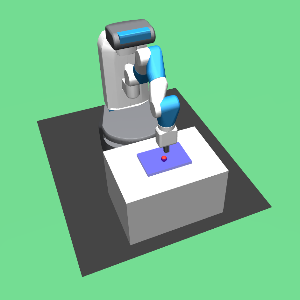
\includegraphics[width=\linewidth]{figures/chapter6/fetch_vol_resize.png}
    \subcaption{Fetch enviroment}
    \label{fig:fetch_volumn}
  \end{subfigure}
  \begin{subfigure}{0.24\columnwidth}
    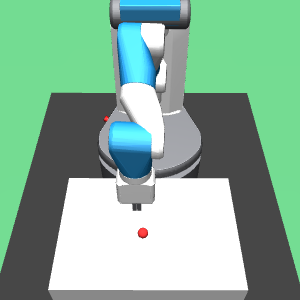
\includegraphics[width=\linewidth]{figures/chapter6/fetch_view.png}
    \subcaption{Fetch visual input}
    \label{fig:fetch_view}
  \end{subfigure}
  \begin{subfigure}{0.24\columnwidth}
    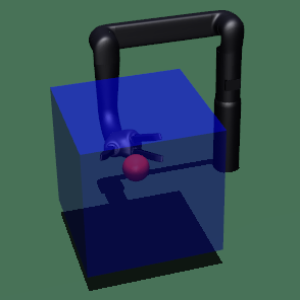
\includegraphics[width=\linewidth]{figures/chapter6/jaco_vol_resize.png}
    \subcaption{Jaco environment}
    \label{fig:jaco_volumn}
  \end{subfigure}
  \begin{subfigure}{0.24\columnwidth}
    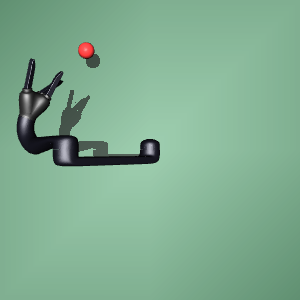
\includegraphics[width=\linewidth]{figures/chapter6/jaco_top.png}
    \subcaption{Jaco visual input}
    \label{fig:jaco_view}
  \end{subfigure}
  \caption[Examples of Fetch and Jaco robot manipulation environments.]{(a) Fetch environment, (b) an example of Fetch visual input, (c) Jaco environment, and (d) an example of Jaco visual input. The blue cuboids indicate the sampling space of the target objects.}
  \label{fig:robot_setups}
\end{figure}

The Fetch robot environment includes a 7 degrees-of-freedom (DOF) robot arm, and it is modified based on the model provided in OpenAI Gym~\cite{plappert2018multi}. In our Fetch environment, we revise the original proprioceptive input, where we delete the velocity and position of the gripper and the position of the target. It now only contains the position and velocity of 7 joints of the robot arm. In order to acquire visual inputs, we also add an extra RGB camera in front of the robot arm (see Figure~\ref{fig:fetch_view}). The control scheme remains the same, which is the relative position of the gripper in $x$, $y$ and $z$ axis. The target object is placed on the table. During training, the position of the target object is randomly sampled in the 2D space (see the blue cuboid in Figure~\ref{fig:fetch_volumn}) of the table surface. During testing, 80 fixed uniformly distributed positions are used to evaluate the performance of the agent.

The Jaco robot environment includes a 6 DoF robot arm (the gripper is disabled). The proprioceptive input contains the position and velocity of 6 joints. An RGB camera is placed on the top of the robot arm to provide visual inputs (see Figure~\ref{fig:jaco_view}). The action space is the 6 joint velocities of the robot arm. During training, the position of the target object is randomly sampled in a 3D space (see the blue cuboid in Figure~\ref{fig:jaco_volumn}). During testing, 250 uniformly distributed fixed positions are used to evaluate the performance of the agent.

The maximum step of each episode is up to 100 in training, which is used to encourage the agent to have enough exploration in the environment. The maximum step of each episode is limited to 20 in testing, which is used to avoid random actions to reach the target. The reward function is similar to Equation~\eqref{eq:sparse_reward}, the agent will achieve a +1 reward if the distance between the gripper and the target is smaller than a threshold $\epsilon$ (in this chapter, $\epsilon=$10cm), otherwise, it only gets 0. More details of these two environments are provided in Table~\ref{tbl:exp_setup}.

\begin{table}[h!]
  \centering
  \begin{tabular}{c|cc}
    \toprule
    Setting & Fetch & Jaco \\
    \midrule
    Active (Total) DoF & 7 (8) & 6 (9) \\
    Target Range & $21 \times 31 \text{cm}^2$ & $40 \times 40 \times 40 \text{cm}^3$ \\
    Num. Test Targets & 80 & 250 \\
    Vision Input & $3 \times 64 \times 64$ & $3 \times 64 \times 64$ \\
    Proprioceptive Inputs & 30 & 18 \\
    Control Type & Position & Velocity \\
    Num. Actions & 3 & 6 \\
    Action Discretisation & 5 & 5 \\
    Control Frequency & 6.67Hz & 6.67Hz \\
    \bottomrule
  \end{tabular}
  \caption{The details of the experimental setup of Fetch and Jaco environments.}
  \label{tbl:exp_setup}
\end{table}

\subsection{Training Configurations}
\begin{figure}[h!]
  \centering
  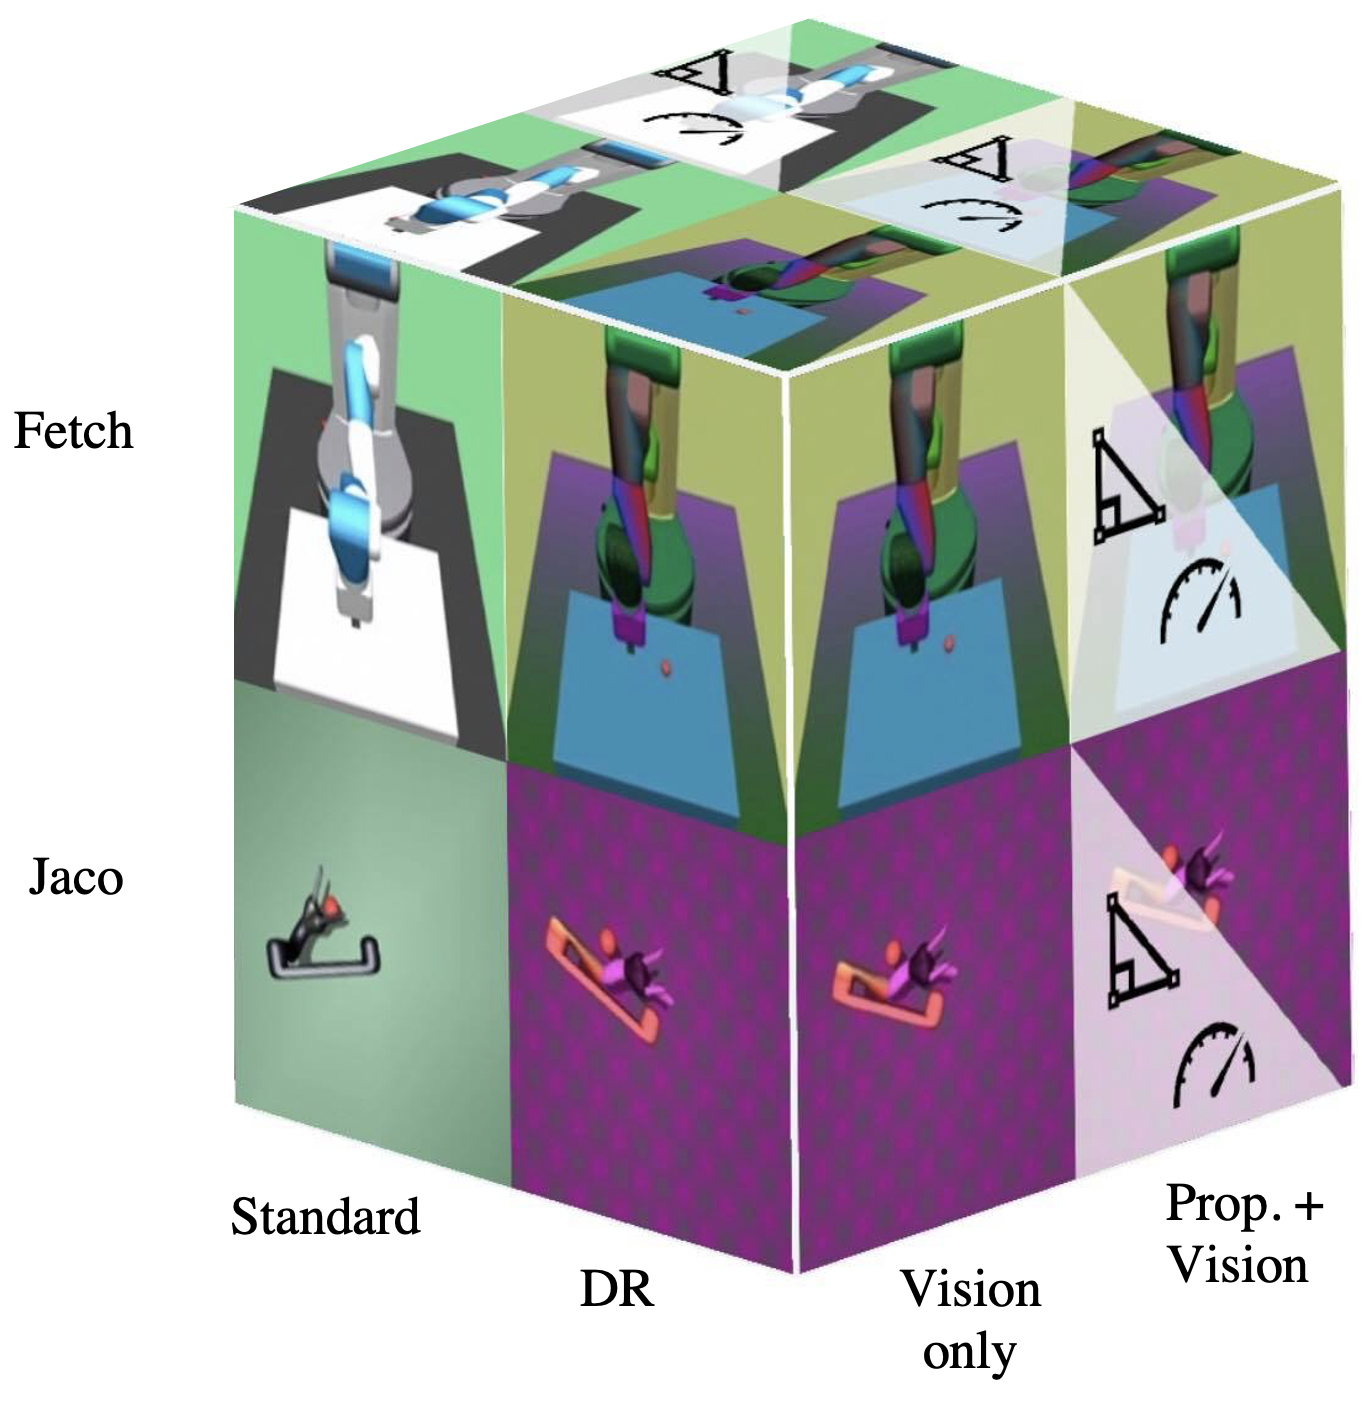
\includegraphics[width=0.85\linewidth]{figures/chapter6/axes.png}
  \caption[Visualisation of 8 different experimental conditions.]{The 8 different experimental conditions: 2 robots (Fetch vs. Jaco), 2 input modalities (vision vs. vision + proprioception), 2 visual conditions (DR vs. no DR). [This diagram was created by Dr.Kai Arulkumaran and Tamara Gerbert~\cite{dai2022analysing}.]}
  \label{fig:axes}
\end{figure}
We setup 8 different configurations to cover different possible training strategies and provide a comprehensive comparison. There are different combinations over three primitives: 1) using Fetch robot arm or Jaco robot arm, 2) using visual input only or visual input + proprioceptive input, and 3) training with or without domain randomisation (DR) (see Figure~\ref{fig:axes}).

{The two robot arms have different morphologies and control schemes. In addition,  we also set different target spaces (2D and 3D) to control the difficulties of the tasks. Thus, we can obtain some indication on whether the results and conclusions are generalised.}

For a real-world deployment, one would want to use as many sensors as feasible. However, we are interested in how the absence of specific input modalities can affect learning, as this changes the way the agent is able to extract information from the environment. For example, while one might expect robots equipped with proprioceptive sensors to use these alone for pose estimation, agents can also learn to utilise vision, if extracting a pose from images is not too difficult.

Finally, analogously to how \emph{data augmentation}~\cite{lecun1998gradient,shorten2019survey} can be used to improve the generalisation of models in supervised learning settings, \emph{domain randomisation} (Figure \ref{fig:dr_example}) is a common training paradigm in ``sim2real'' approaches for learning real-world robots control~\cite{andrychowicz2018learning,james2017transferring,peng2018sim,sadeghi2017cad2rl,tobin2017domain}. In DR, various properties of the simulation are varied, altering anything from the positions or dynamical properties of objects to their visual appearance, resulting in an expansion of the training domain. We therefore test how the agents trained with or without DR differ. In support of previous results, we show that agents trained with DR are more robust to out-of-distribution (OoD) perturbations. In our experiments, we use a standard visual DR setup. At each timestep, we randomise all of the components in the environment by changing/adding different textures, colour gradients, RGB colours, and noise, except for the target object. More details about the DR textures are described in Table~\ref{tbl:random_summary} and visualised in Figure~\ref{fig:random_vis}.

%\subsection{Domain Randomisation}
\begin{table}[h!]
  \centering
  \resizebox{\linewidth}{!}{
  \begin{tabular}{c|c|c}
    \toprule
    No. & Option & Description \\
    \midrule
   1 & checkerboard & Render checkerboard pattern with two random RGB colours\\
   2 & gradient & Render gradient in vertical/horizontal direction with two random RGB colours\\
   3 & flat\_rgb & Render single random RGB colour\\
   4 & noise & Render artificial noise with two random RGB colours\\
    \bottomrule
  \end{tabular}}
   \caption[DR textures used during training.]{DR textures used during training. At every environment timestep, for each component (e.g., robot arm, skybox, table; the Jaco robot has 13 components, and the Fetch robot has 19 components), the appearance of the component is rendered using a sequential sampling process. In the first step of the sampling process, one of each of the 4 possible choices is made with the same probability, then the subsequent appearance of each component is determined by a second draw, described in the rightmost column of the table. Each RGB channel is drawn uniformly from $\{0 \ldots 255\}$. The details of each option are described in Table~\ref{tbl:texture_expression}.}
\label{tbl:random_summary}
\end{table}

\begin{table}[h!]
  \centering
  \resizebox{\linewidth}{!}{
  \begin{tabular}{c|c|c}
    \toprule
    No. & Option & Expression \\
    \midrule
   1 & checkerboard & texture\_mat[x, y] = rgb1 \textbf{if} (x + y) $\%$ 2 == 0 \textbf{else} rgb2\\
   2 & gradient & texture\_mat[x, y] = (1 - p) $\cdot$ rgb1 + p $\cdot$ rgb2, vertical: p = y / (height - 1), horizontal: p = x / (width - 1)\\
   3 & flat\_rgb & texture\_mat[x, y] = rgb1\\
   4 & noise & texture\_mat[x, y] = rgb1 \textbf{if} p $>$ 0.9 \textbf{else} rgb2, p $\sim$ U(0, 1)\\
    \bottomrule
  \end{tabular}
  }
\caption[Python pseudocode describing the DR texture generators.]{Python pseudocode describing the DR texture generators. rgb1 and rgb2 are random RGB colours; the value of each RGB channel is drawn uniformly from $\{0 \ldots 255\}$.}
\label{tbl:texture_expression}
\end{table}

\begin{figure}[h!]
  \centering
  \begin{subfigure}{0.24\columnwidth}
    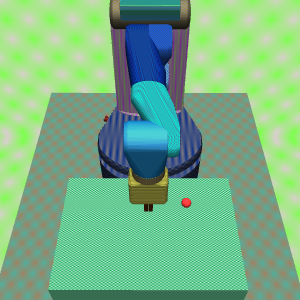
\includegraphics[width=\linewidth]{figures/chapter6/rand_checker.png}
    \subcaption{checkerboard}
  \end{subfigure}
  \begin{subfigure}{0.24\columnwidth}
    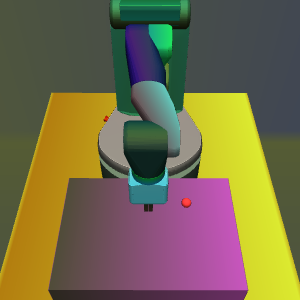
\includegraphics[width=\linewidth]{figures/chapter6/rand_gradient.png}
    \subcaption{gradient}
  \end{subfigure}
  \begin{subfigure}{0.24\columnwidth}
    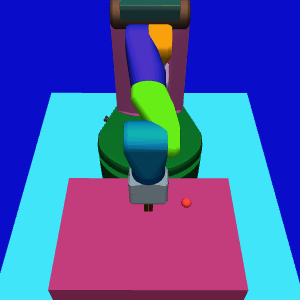
\includegraphics[width=\linewidth]{figures/chapter6/rand_rgb.png}
    \subcaption{flat\_rgb}
  \end{subfigure}
  \begin{subfigure}{0.24\columnwidth}
    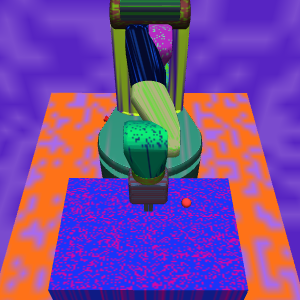
\includegraphics[width=\linewidth]{figures/chapter6/rand_noise.png}
    \subcaption{noise}
  \end{subfigure}
  \caption[Visualisation of different DR textures used during training.]{Visualisation of different DR textures used during training: (a) checkerboard, (b) gradient, (c) flat\_rgb, (d) noise.}
  \label{fig:random_vis}
\end{figure}


\subsection{Network Structure and Training Details}
\begin{figure}[h!]
  \centering
  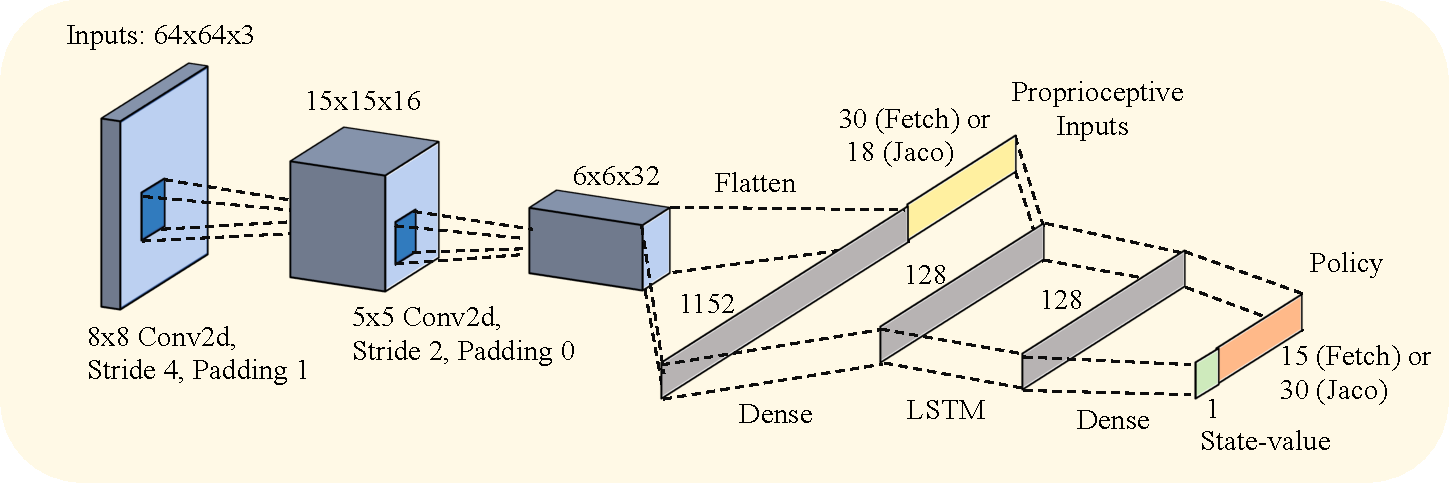
\includegraphics[width=\linewidth]{figures/chapter6/network-arch-td.pdf}
  \caption{The overview of the network architecture used in the experiments.}
  \label{fig:network}
\end{figure}
The network architecture follows the same actor-critic style used in the work of Rusu \textit{et al.}~\cite{rusu2017sim} (see Figure~\ref{fig:network}). The visual input is first passed through 2 convolutional layers, and then the features of the last convolutional layer are flattened into 1152-dimensional vector. Subsequently, if proprioceptive input is provided, it will be concatenated with the previous flatten vector and then sent into a fully connected layer. This is followed by a long short-term memory (LSTM) layer. Finally, the output of the LSTM layer will be sent to two independent fully connected layers to predict the policy $\pi(a_{t}|s_{t};\theta)$ and state value $V(s_{t};\theta)$, respectively. 

In the experiment, proximal policy optimisation (PPO) is used as the base RL algorithm, and 4 MPI workers are used to parallelise the training. During training, each MPI worker uses 8 threads to collect experience for 128 timesteps per epoch. PPO update per epoch is 4 with a batch size equals to 256. Adam is selected as the optimiser, and learning rate is 0.00025. Clip ratio $\epsilon$ is 0.1. Discount factor $\gamma$ is 0.99. A complete training for one model lasts 5000 epochs, and it needs to run on a GTX-1080Ti GPU for one day. For each training configuration, we train the models with 5 different seeds. The overall setup is detailed in Algorithm~\ref{alg:overall_algo}. The code and pretrained models used in this paper are available at: \url{https://github.com/TianhongDai/domain-rand-interp}.

\begin{algorithm}[h!]
\caption{PPO + DR training.}
\label{alg:overall_algo}
\begin{algorithmic}
\REQUIRE environment $E$, actor network $\pi(a|s;\theta)$, critic network $V_{\pi}(s;\theta)$, number of training epochs $N$, number of timesteps to collect data $T$, number of PPO updates $M$, on-policy transition memory $\mathcal{B}$
\FOR{epoch $= 1, 2, \ldots, N$}
  \STATE $\mathcal{B} \gets \varnothing$
  \FOR{$t = 1, 2, \ldots, T$}
    \IF{$E$ has terminated}
      \STATE Reset $E$ and receive DR \indent\indent state $s_0$
    \ENDIF
    \STATE Sample an action $a_t \sim \pi(a|s_t;\theta)$
    \STATE Execute $a_{t}$ in $E$ and receive reward $r_t$, DR next \indent\indent state $s_{t+1}$
    \STATE Store the transition $\left(s_t, a_t, r_t, s_{t+1} \right)$ in $\mathcal{B}$
  \ENDFOR
  \FOR{PPO update $= 1, 2, \cdots, M$}
    \STATE Update $\pi(a|s;\theta)$ using gradient ascent on Eq.\eqref{eq:standard_ppo}  with data from $\mathcal{B}$
    \STATE Update $V_{\pi}(s;\theta)$ using gradient descent on Eq.\eqref{eq:mse} \indent\indent with data from $\mathcal{B}$
  \ENDFOR
\ENDFOR
\end{algorithmic}
\end{algorithm}

\section{Results and Analysis}
\label{ch6:results}
\begin{figure}[h!]
  \centering
  %\hspace{0.025\textwidth}
  \begin{subfigure}{0.49\textwidth}
    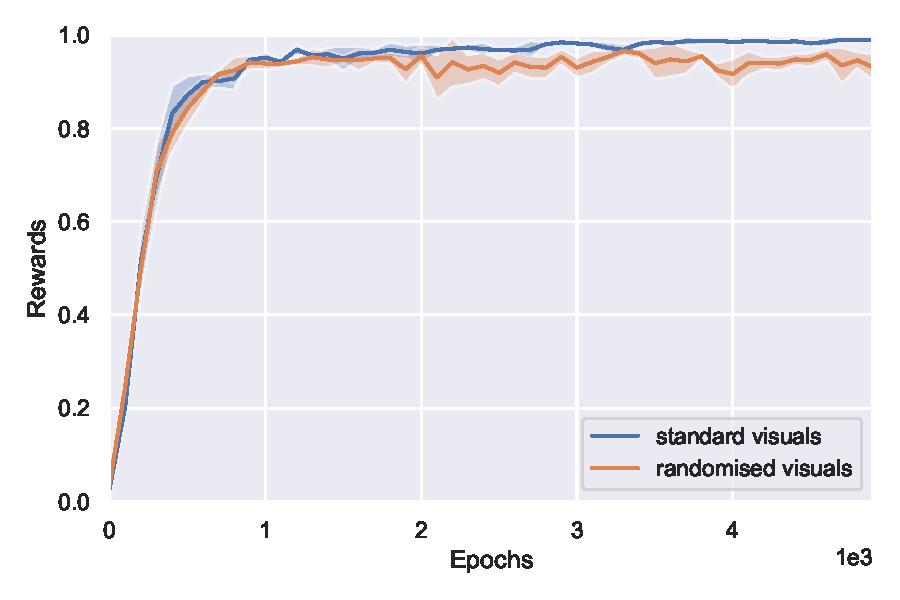
\includegraphics[width=\textwidth]{figures/chapter6/training_curves/jaco_prop.pdf}
    \caption{Trained with Proprioceptive inputs}
  \end{subfigure}\hfill
  \begin{subfigure}{0.49\textwidth}
    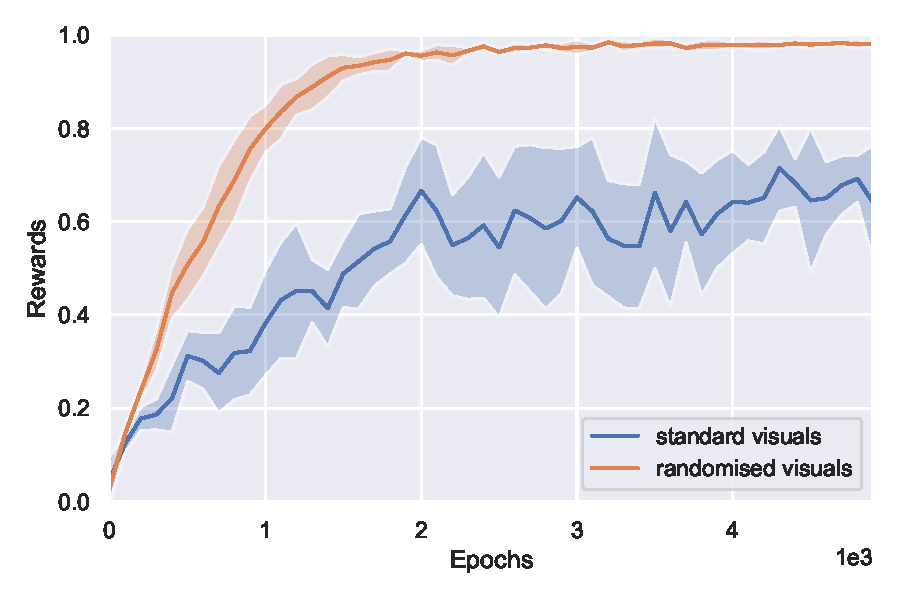
\includegraphics[width=\textwidth]{figures/chapter6/training_curves/jaco_noprop.pdf}
    \caption{Trained without proprioceptive inputs}
  \end{subfigure}
  %\hspace{0.025\textwidth}
  \caption[The learning curves of Jaco agents trained with DR and with or without proprioceptive inputs.]{The learning curves of Jaco agents trained with DR and with (a) or without (b) proprioceptive inputs. (a) the agent have similar performance in both standard and DR environments. (b) the agent has lower performance in standard environment. The solid line is the median value and the shadow area is the 95$\%$ confidence interval.}
  \label{fig:domain_shift}
\end{figure}

Before formally testing and analysing the models, they are fully trained with 8 training configurations and the same hyperparameters to achieve promising performance. However, in the Jaco environment, we also find that the model trained with visual + proprioceptive inputs and DR has a performance degradation when using standard visual inputs (no DR; see Figure~\ref{fig:domain_shift}). This is unexpected when the trained policy is transferred from complex visual scenarios to a simple visual scenario, and this observation demonstrates that this agent is overfitting to DR visual inputs. Since each model has different performance in the standard environment, it is more meaningful to compare the performance variation of individual models under different test conditions.

\subsection{Test Conditions}
\begin{figure*}[h!]
  \centering
  \begin{subfigure}{0.32\textwidth}
    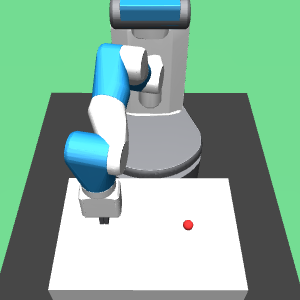
\includegraphics[width=\textwidth]{figures/chapter6/test_observations/standard}
    \caption{Standard}
  \end{subfigure}
  \begin{subfigure}{0.32\textwidth}
    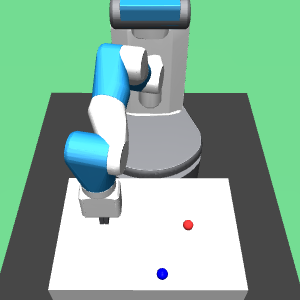
\includegraphics[width=\textwidth]{figures/chapter6/test_observations/colour_b}
    \caption{Colour}
  \end{subfigure}
  \begin{subfigure}{0.32\textwidth}
    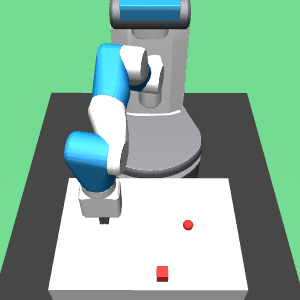
\includegraphics[width=\textwidth]{figures/chapter6/test_observations/shape}
    \caption{Shape}
  \end{subfigure}
  \begin{subfigure}{0.32\textwidth}
    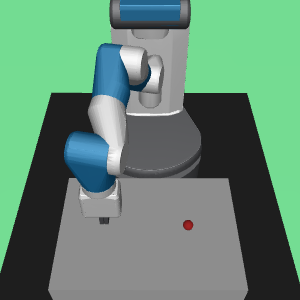
\includegraphics[width=\textwidth]{figures/chapter6/test_observations/illumination}
    \caption{Illumination (Lvl.)}
  \end{subfigure}
  \begin{subfigure}{0.32\textwidth}
    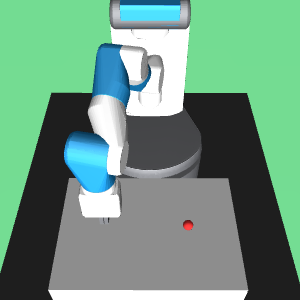
\includegraphics[width=\textwidth]{figures/chapter6/test_observations/illumination_dir}
    \caption{Illumination (Dir.)}
  \end{subfigure}
  \begin{subfigure}{0.32\textwidth}
    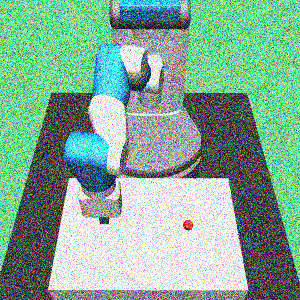
\includegraphics[width=\textwidth]{figures/chapter6/test_observations/noise}
    \caption{Noise}
  \end{subfigure}
  \begin{subfigure}{0.32\textwidth}
    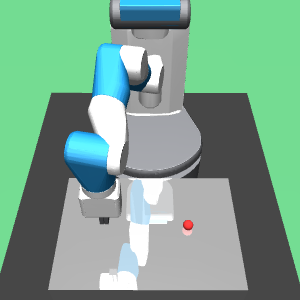
\includegraphics[width=\textwidth]{figures/chapter6/test_observations/reflection}
    \caption{Reflection}
  \end{subfigure}
  \begin{subfigure}{0.32\textwidth}
    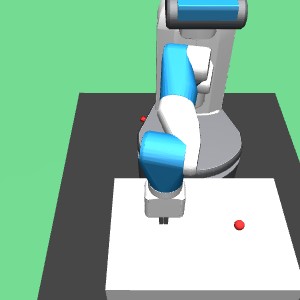
\includegraphics[width=\textwidth]{figures/chapter6/test_observations/translation}
    \caption{Translation}
  \end{subfigure}
  \begin{subfigure}{0.32\textwidth}
    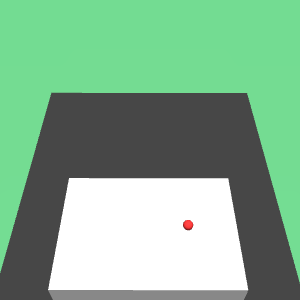
\includegraphics[width=\textwidth]{figures/chapter6/test_observations/invisible}
    \caption{Invisibility}
  \end{subfigure}
  \caption[The visualisation of different test conditions in the Fetch environment.]{The visualisation of different test conditions in the Fetch environment. The agents are trained only in the standard condition. There are no extra distractors introduced during training.}
  \label{fig:tests}
\end{figure*}
We develop 8 different test conditions to evaluate the generalisation ability of the trained agents. Figure~\ref{fig:tests} shows an overview of 8 test conditions in the Fetch environment. The details of each test condition are listed below:
\begin{enumerate}
\item[a)] \textbf{Standard}: This is the default setting of the environment, which is used to evaluate the baseline performance of the agent for further comparison. 

\item[b)] \textbf{Colour}: This condition introduces a distractor object, which has the same shape and size as the target object but has a different colour. It aims to evaluate the robustness of the agent when there exists an extra object with different colours. We use five different colours: yellow, blue, green, brown and purple. Some of these colours have a red component (yellow, brown and purple), while others do not (blue and green).

\item[c)] \textbf{Shape}: This condition introduces a red distractor object, which has a different shape to the target object. It aims to evaluate the robustness of the agent when there exists an extra object with different shapes. We use four different shapes: cube, ellipsoid, rectangle and diamond.

\item[d)] \textbf{Illumination (Lvl.)}: This condition changes the diffuse intensity of the source of light. We use five illumination levels: 0.4 to 0.0 for the Fetch environment, and 0.9 to 0.1 for the Jaco environment.

\item[e)] \textbf{Illumination (Dir.)}: This condition changes the location of the source of light. We use five different locations for both Fetch and Jaco environments.

\item[f)] \textbf{Noise}: This condition adds Gaussian noise $\mathcal{N}(0, 0.25)$ to the visual inputs. This noise is not the same as the one generated in DR.

\item[g)] \textbf{Reflection}: This condition makes the table of the Fetch environment and the floor of the Jaco environment reflective, and it can produce mirror-like reflections in these surfaces.

\item[h)] \textbf{Translation}: This condition shifts the RGB camera's location. We use 5 locations: -20 to 20cm in the $y$ direction for the Fetch environment, and -20 to 20cm in the $x$ direction for the Jaco environment.

\item[i)] \textbf{Invisibility}: This condition is an extreme case, where the robot arm becomes transparent, and it is only used to investigate the importance of the visual inputs to localise the robot arm.
\end{enumerate}

\subsection{Quantitative Results on Testing Conditions}
We first discuss how local visual changes affect the performance of these trained agents. Table~\ref{tbl:tests} demonstrates the performance of agents with different training configurations under different test conditions. For both the Fetch and Jaco environments, the agents trained with DR perform slightly worse than those trained without DR in the standard test condition. However, agents trained with DR show strong robustness to both kinds of distractors. In Table~\ref{tbl:diff_colours}, we also provide the performance of the agents to different colours and different shapes of the distractors.

\begin{table}[h]
%\begin{sidewaystable}[h!]
  %\label{tbl:tests}
  \resizebox{\linewidth}{!}{
  \begin{tabular}{c|cc|c|cc|cc|ccc|c}
    \toprule
    Robot & DR & Prop. & Standard & Colours & Shapes & Illum (Lvl.) & Illum (Dir.) & Noise & Reflection & Translation & Invisibility\\
    \midrule
    Fetch & {\xmark}   & {\xmark}   & 1.00$\pm 0.00$ & 0.99$\pm 0.00$ & 0.83$\pm 0.06$ & 0.69$\pm 0.05$ & 0.54$\pm 0.07$ & 0.98$\pm 0.00$ & 0.45$\pm 0.04$ & 0.27$\pm 0.08$ & 0.00$\pm 0.00$\\
    Fetch & {\xmark}   & {\cmark} & 1.00$\pm 0.00$ & 0.94$\pm 0.08$ & 0.52$\pm 0.09$ & 0.59$\pm 0.06$ & 0.49$\pm 0.07$ & 0.99$\pm 0.00$ & 0.57$\pm 0.08$ & 0.23$\pm 0.08$ & 0.00$\pm 0.00$\\
    Fetch & {\cmark} & {\xmark}   & 0.98$\pm 0.00$ & 0.97$\pm 0.00$ & 0.94$\pm 0.02$ & 0.96$\pm 0.01$ & 0.74$\pm 0.06$ & 0.99$\pm 0.01$ & 0.97$\pm 0.01$ & 0.48$\pm 0.06$ & 0.00$\pm 0.00$\\
    Fetch & {\cmark} & {\cmark} & 1.00$\pm 0.00$ & 1.00$\pm 0.00$ & 0.98$\pm 0.01$ & 0.99$\pm 0.00$ & 0.88$\pm 0.04$ & 0.97$\pm 0.01$ & 0.99$\pm 0.01$ & 0.54$\pm 0.06$ & 0.02$\pm 0.02$\\
    \hline
    Jaco  & {\xmark}   & {\xmark}   & 1.00$\pm 0.00$ & 0.77$\pm 0.06$ & 0.37$\pm 0.07$ & 0.97$\pm 0.01$ & 0.84$\pm 0.04$ & 0.64$\pm 0.03$ & 0.73$\pm 0.03$ & 0.56$\pm 0.06$ & 0.00$\pm 0.00$\\
    Jaco  & {\xmark} & {\cmark} & 1.00$\pm 0.00$ & 0.81$\pm 0.04$ & 0.38$\pm 0.06$ & 0.88$\pm 0.03$ & 0.91$\pm 0.01$ & 0.48$\pm 0.06$ & 0.62$\pm 0.06$ & 0.69$\pm 0.05$ & 0.00$\pm 0.00$\\
    Jaco  & {\cmark} & {\xmark}   & 0.65$\pm 0.06$ & 0.65$\pm 0.02$ & 0.59$\pm 0.03$ & 0.64$\pm 0.03$ & 0.55$\pm 0.03$ & 0.58$\pm 0.04$ & 0.43$\pm 0.06$ & 0.31$\pm 0.04$ & 0.01$\pm 0.00$\\
    Jaco  & {\cmark} & {\cmark} & 0.99$\pm 0.00$ & 0.99$\pm 0.00$ & 0.84$\pm 0.06$ & 0.82$\pm 0.04$ & 0.88$\pm 0.03$ & 0.90$\pm 0.01$ & 0.95$\pm 0.01$ & 0.66$\pm 0.05$ & 0.92$\pm 0.02$\\
    \bottomrule
  \end{tabular}}
  \caption[Test performance of all models under different test conditions.]{Test performance of all models with local visual changes (distractors), global visual changes, and invisibility (visual pose estimation test). Colour and shape results are averaged over 9 different distractor locations, as well as all colours and shapes, respectively. Checkmarks and crosses indicate enabling/disabling DR and proprioceptive inputs (Prop.), respectively. Mean $\pm$ standard error are calculated over all models (seeds) and test target locations.}
  \label{tbl:tests}
%\end{sidewaystable}
\end{table}

In the Fetch environment, the trained agents are more robust to the colour distractors. However, the shape distractors decrease the performance of the agents trained without DR, especially for agents trained with proprioceptive inputs and without DR, which reduces the success rate by 0.48 (the relative changes in its performance in the standard test environment, which is 1.00$\pm$0.00; see Table~\ref{tbl:tests}). This implies that the agent trained with proprioceptive inputs and without DR localises the target object primarily by colour information and partly with shape information. The agent trained with visual inputs and without DR merely drops 0.17 success rate (the relative changes in its performance in the standard test environment, which is 1.00$\pm$0.00; see Table~\ref{tbl:tests}). This is because the agent trained with only visual inputs requires better representation/feature learning to estimate the pose of the robot arm (i.e., self-localisation), and these learned features can help the agent to distinguish between different shapes and colours.

In the Jaco environment, both agents trained without DR show performance degradation when there exists a distractor with red components, and both agents trained with DR have significant performance drops when the shape of the distractor is a diamond, which has a similar appearance to a sphere in a low-resolution viewed input. It also indicates that the agents trained without DR prefer to localise the target object via red colour.

In addition, we also test the effect of the distractors on the agent in different positions. In Table~\ref{tbl:vary_distractor}, it only has a few influences on performance.

% \begin{table}[H]
% %\begin{sidewaystable}[h!]
%   %\label{tbl:tests}
%   \resizebox{\linewidth}{!}{
%   \begin{tabular}{c|cc|c|cc|cc|ccc|c}
%     \toprule
%     Robot & DR & Prop. & Standard & Colours & Shapes & Illumination (Lvl.) & Illumination (Dir.) & Noise & Reflection & Translation & Invisibility\\
%     \midrule
%     Fetch & {\xmark}   & {\xmark}   & 1.000$\pm 0.000$ & 0.993$\pm 0.004$ & 0.827$\pm 0.056$ & 0.694$\pm 0.049$ & 0.539$\pm 0.069$ & 0.980$\pm 0.006$ & 0.447$\pm 0.039$ & 0.270$\pm 0.079$ & 0.000$\pm 0.000$\\
%     Fetch & {\xmark}   & {\cmark} & 1.000$\pm 0.000$ & 0.937$\pm 0.027$ & 0.524$\pm 0.087$ & 0.593$\pm 0.064$ & 0.491$\pm 0.066$ & 0.988$\pm 0.004$ & 0.570$\pm 0.078$ & 0.231$\pm 0.078$ & 0.000$\pm 0.000$\\
%     Fetch & {\cmark} & {\xmark}   & 0.983$\pm 0.004$ & 0.974$\pm 0.004$ & 0.939$\pm 0.018$ & 0.957$\pm 0.008$ & 0.740$\pm 0.058$ & 0.985$\pm 0.007$ & 0.972$\pm 0.011$ & 0.480$\pm 0.064$ & 0.000$\pm 0.000$\\
%     Fetch & {\cmark} & {\cmark} & 0.997$\pm 0.002$ & 0.997$\pm 0.001$ & 0.978$\pm 0.009$ & 0.992$\pm 0.002$ & 0.883$\pm 0.038$ & 0.970$\pm 0.008$ & 0.985$\pm 0.005$ & 0.536$\pm 0.063$ & 0.023$\pm 0.015$\\
%     \hline
%     Jaco  & {\xmark}   & {\xmark}   & 0.995$\pm 0.003$ & 0.772$\pm 0.058$ & 0.367$\pm 0.069$ & 0.966$\pm 0.012$ & 0.838$\pm 0.035$ & 0.635$\pm 0.028$ & 0.734$\pm 0.032$ & 0.556$\pm 0.063$ & 0.000$\pm 0.000$\\
%     Jaco  & {\xmark} & {\cmark} & 0.995$\pm 0.001$ & 0.808$\pm 0.044$ & 0.382$\pm 0.064$ & 0.876$\pm 0.032$ & 0.911$\pm 0.014$ & 0.478$\pm 0.059$ & 0.618$\pm 0.061$ & 0.688$\pm 0.048$ & 0.001$\pm 0.001$\\
%     Jaco  & {\cmark} & {\xmark}   & 0.650$\pm 0.056$ & 0.652$\pm 0.022$ & 0.593$\pm 0.031$ & 0.643$\pm 0.027$ & 0.549$\pm 0.032$ & 0.575$\pm 0.040$ & 0.429$\pm 0.060$ & 0.310$\pm 0.041$ & 0.007$\pm 0.002$\\
%     Jaco  & {\cmark} & {\cmark} & 0.991$\pm 0.004$ & 0.989$\pm 0.002$ & 0.843$\pm 0.061$ & 0.816$\pm 0.043$ & 0.882$\pm 0.031$ & 0.896$\pm 0.007$ & 0.946$\pm 0.006$ & 0.658$\pm 0.054$ & 0.916$\pm 0.022$\\
%     \bottomrule
%   \end{tabular}}
%   \caption[Test performance of all models under different test conditions.]{Test performance of all models with local visual changes (distractors), global visual changes, and invisibility (visual pose estimation test). Colour and shape results are averaged over 9 different distractor locations, as well as all colours and shapes, respectively. Checkmarks and crosses indicate enabling/disabling DR and proprioceptive inputs (Prop.), respectively. Mean $\pm$ standard error are calculated over all models (seeds) and test target locations.}
%   \label{tbl:tests}
% %\end{sidewaystable}
% \end{table}

% \begin{table}[h!]
% %\begin{sidewaystable}[h!]
%   \resizebox{\linewidth}{!}{
%   \begin{tabular}{c|cc|ccccc|cccc}
%     \toprule
%     Robot & DR & Prop. & Yellow & Blue & Green & Brown & Purple & Cube & Ellipsoid & Rectangle & Diamond\\
%     \midrule
%     Fetch & {\xmark}   & {\xmark}   & 0.993$\pm 0.007$ & 1.000$\pm 0.000$ & 1.000$\pm 0.000$ & 0.978$\pm 0.017$ & 0.995$\pm 0.004$ & 0.775$\pm 0.085$ & 0.993$\pm 0.007$ & 0.960$\pm 0.036$ & 0.580$\pm 0.142$\\
%     Fetch & {\xmark}   & {\cmark} & 0.875$\pm 0.088$ & 1.000$\pm 0.000$ & 1.000$\pm 0.000$ & 0.825$\pm 0.069$ & 0.983$\pm 0.006$ & 0.243$\pm 0.064$ & 0.980$\pm 0.006$ & 0.783$\pm 0.079$ & 0.090$\pm 0.048$\\
%     Fetch & {\cmark} & {\xmark}   & 0.970$\pm 0.011$ & 0.980$\pm 0.006$ & 0.975$\pm 0.006$ & 0.973$\pm 0.010$ & 0.973$\pm 0.011$ & 0.913$\pm 0.042$ & 0.975$\pm 0.009$ & 0.965$\pm 0.013$ & 0.905$\pm 0.048$\\
%     Fetch &{\cmark} & {\cmark} & 0.995$\pm 0.003$ & 0.998$\pm 0.002$ & 1.000$\pm 0.000$ & 0.998$\pm 0.002$ & 0.995$\pm 0.003$ & 0.963$\pm 0.020$ & 0.998$\pm 0.002$ & 0.995$\pm 0.003$ & 0.958$\pm 0.022$\\
%     \hline
%     Jaco  & {\xmark}   & {\xmark}   & 0.281$\pm 0.067$ & 0.871$\pm 0.036$ & 0.994$\pm 0.003$ & 0.730$\pm 0.095$ & 0.984$\pm 0.008$ & 0.274$\pm 0.077$ & 0.407$\pm 0.098$ & 0.759$\pm 0.066$ & 0.027$\pm 0.006$\\
%     Jaco  & {\xmark}   & {\cmark} & 0.451$\pm 0.040$ & 0.941$\pm 0.032$ & 0.993$\pm 0.002$ & 0.706$\pm 0.064$ & 0.950$\pm 0.028$ & 0.258$\pm 0.044$ & 0.440$\pm 0.058$ & 0.784$\pm 0.044$ & 0.045$\pm 0.009$\\
%     Jaco  & {\cmark} & {\xmark}   & 0.640$\pm 0.046$ & 0.655$\pm 0.055$ & 0.651$\pm 0.055$ & 0.668$\pm 0.046$ & 0.648$\pm 0.046$ & 0.636$\pm 0.040$ & 0.642$\pm 0.035$ & 0.666$\pm 0.047$ & 0.426$\pm 0.054$\\
%     Jaco  & {\cmark} & {\cmark} & 0.987$\pm 0.005$ & 0.990$\pm 0.003$ & 0.987$\pm 0.003$ & 0.990$\pm 0.003$ & 0.990$\pm 0.003$ & 0.970$\pm 0.017$ & 0.970$\pm 0.011$ & 0.990$\pm 0.003$ & 0.441$\pm 0.128$\\
%     \bottomrule
%   \end{tabular}}
%   \caption[Test performance of all models with local visual changes.]{Test performance of all models with local visual changes (distractors). Checkmarks and crosses indicate enabling/disabling DR and proprioceptive inputs (Prop.), respectively. Mean $\pm$ standard error are calculated over all models (seeds), test target locations, and 9 distractor locations.}
%   \label{tbl:diff_colours}
% %\end{sidewaystable}
% \end{table}

\begin{table}[h!]
%\begin{sidewaystable}[h!]
  \resizebox{\linewidth}{!}{
  \begin{tabular}{c|cc|ccccc|cccc}
    \toprule
    Robot & DR & Prop. & Yellow & Blue & Green & Brown & Purple & Cube & Ellipsoid & Rectangle & Diamond\\
    \midrule
    Fetch & {\xmark}   & {\xmark}   & 0.99$\pm 0.01$ & 1.00$\pm 0.00$ & 1.00$\pm 0.00$ & 0.98$\pm 0.02$ & 1.00$\pm 0.00$ & 0.78$\pm 0.09$ & 0.99$\pm 0.01$ & 0.96$\pm 0.04$ & 0.58$\pm 0.14$\\
    Fetch & {\xmark}   & {\cmark} & 0.88$\pm 0.09$ & 1.00$\pm 0.00$ & 1.00$\pm 0.00$ & 0.83$\pm 0.07$ & 0.98$\pm 0.01$ & 0.24$\pm 0.06$ & 0.98$\pm 0.01$ & 0.78$\pm 0.08$ & 0.09$\pm 0.05$\\
    Fetch & {\cmark} & {\xmark}   & 0.97$\pm 0.01$ & 0.98$\pm 0.01$ & 0.98$\pm 0.01$ & 0.97$\pm 0.01$ & 0.97$\pm 0.01$ & 0.91$\pm 0.04$ & 0.98$\pm 0.01$ & 0.97$\pm 0.01$ & 0.91$\pm 0.05$\\
    Fetch &{\cmark} & {\cmark} & 1.00$\pm 0.00$ & 1.00$\pm 0.00$ & 1.00$\pm 0.00$ & 1.00$\pm 0.00$ & 1.00$\pm 0.00$ & 0.96$\pm 0.02$ & 1.00$\pm 0.00$ & 1.00$\pm 0.00$ & 0.96$\pm 0.02$\\
    \hline
    Jaco  & {\xmark}   & {\xmark} & 0.28$\pm 0.07$ & 0.87$\pm 0.04$ & 0.99$\pm 0.00$ & 0.73$\pm 0.10$ & 0.98$\pm 0.01$ & 0.27$\pm 0.08$ & 0.41$\pm 0.10$ & 0.76$\pm 0.07$ & 0.03$\pm 0.01$\\
    Jaco  & {\xmark}   & {\cmark} & 0.45$\pm 0.04$ & 0.94$\pm 0.03$ & 0.99$\pm 0.00$ & 0.71$\pm 0.06$ & 0.95$\pm 0.03$ & 0.26$\pm 0.04$ & 0.44$\pm 0.06$ & 0.78$\pm 0.04$ & 0.05$\pm 0.01$\\
    Jaco  & {\cmark} & {\xmark}   & 0.64$\pm 0.05$ & 0.66$\pm 0.06$ & 0.65$\pm 0.06$ & 0.67$\pm 0.05$ & 0.65$\pm 0.05$ & 0.64$\pm 0.04$ & 0.64$\pm 0.04$ & 0.67$\pm 0.05$ & 0.43$\pm 0.05$\\
    Jaco  & {\cmark} & {\cmark} & 0.99$\pm 0.01$ & 0.99$\pm 0.00$ & 0.99$\pm 0.00$ & 0.99$\pm 0.00$ & 0.99$\pm 0.00$ & 0.97$\pm 0.02$ & 0.97$\pm 0.01$ & 0.99$\pm 0.00$ & 0.44$\pm 0.13$\\
    \bottomrule
  \end{tabular}}
  \caption[Test performance of all models with local visual changes.]{Test performance of all models with local visual changes (distractors). Checkmarks and crosses indicate enabling/disabling DR and proprioceptive inputs (Prop.), respectively. Mean $\pm$ standard error are calculated over all models (seeds), test target locations, and 9 distractor locations.}
  \label{tbl:diff_colours}
%\end{sidewaystable}
\end{table}

\begin{table}[H]
  \centering
  \begin{tabular}{c|cc|cc}
    \toprule
    Robot & DR & Prop. & Colours & Shapes\\
    \midrule
    Fetch & {\xmark}   & {\xmark}   & 0.993$\pm 0.004$ & 0.567$\pm 0.047$\\
    Fetch & {\xmark}   & {\cmark} & 0.937$\pm 0.027$ & 0.507$\pm 0.047$\\
    Fetch & {\cmark} & {\xmark}   & 0.974$\pm 0.004$ & 0.639$\pm 0.051$\\
    Fetch & {\cmark} & {\cmark} & 0.997$\pm 0.001$ & 0.622$\pm 0.050$\\
    \hline
    Jaco  & {\xmark} & {\xmark}   & 0.772$\pm 0.058$ & 0.880$\pm 0.007$\\
    Jaco  & {\xmark} & {\cmark} & 0.808$\pm 0.044$ & 0.897$\pm 0.007$\\
    Jaco  & {\cmark} & {\xmark}   & 0.652$\pm 0.022$ & 0.759$\pm 0.004$\\
    Jaco  & {\cmark} & {\cmark} & 0.989$\pm 0.002$ & 0.930$\pm 0.004$\\
    \bottomrule
  \end{tabular}
  \caption[Test performance of a single model with the distractor presented in 9 different locations.]{Test performance of a single model with distractors locations varying over 9 different on the ground plane (Jaco) and table (Fetch). Checkmarks and crosses indicate enabling/disabling DR and proprioceptive inputs (Prop.), respectively. Mean $\pm$ standard error are calculated for the best model (seed), over all test target locations and all distractor locations.}
  \label{tbl:vary_distractor}
\end{table}


Next, we discuss how global visual changes affect the performance of these trained agents. From Table~\ref{tbl:tests}, in this case, the agents trained with DR show better robustness but still sacrifice a lot of performance in many test conditions.

In the Illumination (Lvl.) condition, the performance of all trained agents decreases as the light intensity reduces ({see Table~\ref{tbl:diff_levels}}). In the Fetch environment, the agents trained with DR are more robust to variations of the illumination intensity. In the Jaco environment, however, the agents trained without proprioception are more robust in this case, compared to agents trained with. This is probably because, in the Jaco environment, the agents trained without proprioception require a more complex visual system for the pose estimation, whereas a simpler visual system can be disrupted by a reduction in contrast or even just a change in the pixel value of the target. Thus the learned features are more robust to the change of the illumination in the environment.
%must learn better features for pose estimation, thus the learned features are more robust to the change of the illumination in the environment.}

In the Illumination (Dir.) condition, the performance of all agents decreases as the direction of the light source changes (see Table~\ref{tbl:diff_dirs}). Similarly, in the Fetch environment, the agents trained with DR are more robust. However, in the Jaco environment, compared to training with DR, providing proprioceptive inputs would be more helpful in this case. 

\begin{table}[H]
\centering
  \resizebox{0.9\linewidth}{!}{
  \begin{tabular}{c|cc|ccccc}
    \toprule
    Robot & DR & Prop. & 0.0/0.1 & 0.1/0.3 & 0.2/0.5 & 0.3/0.7 & 0.4/0.9 \\
    \midrule
    Fetch & {\xmark}   & {\xmark}   & 0.468$\pm 0.670$ & 0.513$\pm 0.081$ & 0.643$\pm 0.076$ & 0.860$\pm 0.047$ & 0.988$\pm 0.009$ \\
    Fetch & {\xmark}   & {\cmark} & 0.325$\pm 0.115$ & 0.383$\pm 0.112$ & 0.508$\pm 0.110$ & 0.775$\pm 0.069$ & 0.973$\pm 0.013$ \\
    Fetch & {\cmark} & {\xmark}   & 0.893$\pm 0.013$ & 0.948$\pm 0.018$ & 0.975$\pm 0.004$ & 0.985$\pm 0.004$ & 0.983$\pm 0.004$ \\
    Fetch & {\cmark} & {\cmark} & 0.983$\pm 0.006$ & 0.990$\pm 0.002$ & 0.995$\pm 0.003$ & 0.995$\pm 0.003$ & 0.995$\pm 0.003$ \\
    \hline
    Jaco  & {\xmark} & {\xmark}   & 0.874$\pm 0.034$ & 0.972$\pm 0.008$ & 0.990$\pm 0.001$ & 0.996$\pm 0.001$ & 0.996$\pm 0.001$ \\
    Jaco  & {\xmark} & {\cmark} & 0.587$\pm 0.043$ & 0.846$\pm 0.022$ & 0.966$\pm 0.007$ & 0.989$\pm 0.002$ & 0.994$\pm 0.001$ \\
    Jaco  & {\cmark} & {\xmark}   & 0.473$\pm 0.049$ & 0.626$\pm 0.042$ & 0.707$\pm 0.039$ & 0.711$\pm 0.046$ & 0.698$\pm 0.041$ \\
    Jaco  & {\cmark} & {\cmark} & 0.442$\pm 0.018$ & 0.713$\pm 0.013$ & 0.946$\pm 0.012$ & 0.986$\pm 0.002$ & 0.994$\pm 0.002$ \\
    \bottomrule
  \end{tabular}}
  \caption[Test performance of all models with different global illumination intensities.]{Test performance of all models with different global illumination intensities; illumination is specificied as Fetch/Jaco. Checkmarks and crosses indicate enabling/disabling DR and proprioceptive inputs (Prop.), respectively. Mean $\pm$ standard error are calculated over all models (seeds) and test target locations.}
  \centering
  \label{tbl:diff_levels}
\end{table}

\begin{table}[H]
 \centering
  \resizebox{0.9\linewidth}{!}{
  \begin{tabular}{c|cc|ccccc}
    \toprule
    Robot & DR & Prop. & 0.0,0.0,-1.0/ & -1.0,0.0,0.0/ & -1.0,0.0,-1.0/ & 0.0,-1.0,0.0/ & 0.0,1.0,1.0/   \\
          &    &       & 0.0,0.0,-1.3  & -1.3,0.0,0.0  & -1.3,0.0,-1.3  & 0.0,-1.3,-1.3 & -1.3,-1.3,-1.3 \\
    \midrule
    Fetch & {\xmark}   & {\xmark}   & 1.000$\pm 0.000$ & 0.020$\pm 0.004$ & 0.593$\pm 0.095$ & 0.518$\pm 0.091$ & 0.563$\pm 0.066$ \\
    Fetch & {\xmark}   & {\cmark} & 1.000$\pm 0.000$ & 0.068$\pm 0.041$ & 0.493$\pm 0.074$ & 0.453$\pm 0.079$ & 0.440$\pm 0.066$ \\
    Fetch & {\cmark} & {\xmark}   & 0.983$\pm 0.004$ & 0.338$\pm 0.117$ & 0.850$\pm 0.087$ & 0.763$\pm 0.097$ & 0.765$\pm 0.075$ \\
    Fetch & {\cmark} & {\cmark} & 0.998$\pm 0.002$ & 0.540$\pm 0.076$ & 0.948$\pm 0.025$ & 0.985$\pm 0.009$ & 0.945$\pm 0.021$ \\
    \hline
    Jaco  & {\xmark}   & {\xmark}   & 0.995$\pm 0.003$ & 0.818$\pm 0.022$ & 0.650$\pm 0.121$ & 0.805$\pm 0.044$ & 0.922$\pm 0.015$ \\
    Jaco  & {\xmark}   & {\cmark} & 0.995$\pm 0.001$ & 0.852$\pm 0.019$ & 0.930$\pm 0.029$ & 0.855$\pm 0.023$ & 0.922$\pm 0.011$ \\
    Jaco  & {\cmark} & {\xmark}   & 0.650$\pm 0.056$ & 0.608$\pm 0.044$ & 0.455$\pm 0.070$ & 0.506$\pm 0.068$ & 0.529$\pm 0.074$ \\
    Jaco  & {\cmark} & {\cmark} & 0.991$\pm 0.004$ & 0.586$\pm 0.017$ & 0.932$\pm 0.016$ & 0.968$\pm 0.010$ & 0.934$\pm 0.016$ \\
    \bottomrule
  \end{tabular}}
  \caption[Test performance of all models with different main illumination directions.]{Test performance of all models with different main illumination directions; direction is specified as Fetch/Jaco. Checkmarks and crosses indicate enabling/disabling DR and proprioceptive inputs (Prop.), respectively. Mean $\pm$ standard error are calculated over all models (seeds) and test target locations.}
  \centering
  \label{tbl:diff_dirs}
\end{table}

For the case of additive Gaussian noise, the agents trained in the Fetch environment are all robust to the noise. However, in the Jaco environment, the agents trained without DR have approximately 30$\%$ performance drop, while the agents with DR only have 10$\%$ performance drop. Although both environments share the same training configurations, either the difficulty of the task or visual layout can make the Fetch agents be more robust to noise than Jaco agents.

In the reflection condition, the agents trained with DR are generally robust. In the Fetch environment, the performance of the agents trained without DR is decreased by 50$\%$. In the Jaco environment, it only causes a minor influence on the performance of the agents trained without DR. One possible explanation is the difference in the sizes of the robot arms. The Jaco robot arm is relatively small in the simulation, so its reflection has insignificant changes in the visual inputs. When the proprioceptive inputs are provided, both Jaco and Fetch agents trained with DR demonstrate better robustness to the changes.

In the translation condition, the performance of all agents is greatly reduced. In the Fetch environment, just as before, agents trained with DR exhibit better robustness. In the Jaco environment, all agents have similar performance, which reflects that these agents are able to learn the extent of translation invariance for the policies. This could be a benefit for the target reaching task in a 3D space, which leads to a more generalisable spatial representation. Performance drops monotonically with deviation from the original location (see Table~\ref{tbl:diff_trans}). The drop is symmetric for the Fetch agents, but asymmetric for the Jaco agents -- a relative shift in the target towards the centre of the image input is better than a shift away.

\begin{table}[H]
 \centering
  \resizebox{\linewidth}{!}{
  \begin{tabular}{c|cc|ccccc}
    \toprule
    Robot & DR & Prop. & -20cm & -10cm & 0cm & 10cm & 20cm \\
    \midrule
    Fetch & {\xmark}   & {\xmark}   & 0.013$\pm 0.004$ & 0.168$\pm 0.101$ & 1.000$\pm 0.000$ & 0.163$\pm 0.091$ & 0.008$\pm 0.004$ \\
    Fetch & {\xmark}   & {\cmark} & 0.043$\pm 0.027$ & 0.075$\pm 0.039$ & 1.000$\pm 0.000$ & 0.035$\pm 0.010$ & 0.000$\pm 0.000$ \\
    Fetch & {\cmark} & {\xmark}   & 0.268$\pm 0.042$ & 0.625$\pm 0.056$ & 0.983$\pm 0.004$ & 0.433$\pm 0.056$ & 0.093$\pm 0.040$ \\
    Fetch & {\cmark} & {\cmark} & 0.358$\pm 0.051$ & 0.685$\pm 0.033$ & 0.998$\pm 0.002$ & 0.488$\pm 0.094$ & 0.153$\pm 0.055$ \\
    \hline
    Jaco  & {\xmark}   & {\xmark}   & 0.107$\pm 0.030$ & 0.570$\pm 0.065$ & 0.995$\pm 0.003$ & 0.714$\pm 0.022$ & 0.394$\pm 0.055$ \\
    Jaco  & {\xmark}   & {\cmark} & 0.464$\pm 0.062$ & 0.826$\pm 0.026$ & 0.995$\pm 0.001$ & 0.757$\pm 0.022$ & 0.399$\pm 0.040$ \\
    Jaco  & {\cmark} & {\xmark}   & 0.175$\pm 0.025$ & 0.265$\pm 0.049$ & 0.650$\pm 0.056$ & 0.321$\pm 0.030$ & 0.141$\pm 0.034$ \\
    Jaco  & {\cmark} & {\cmark} & 0.338$\pm 0.034$ & 0.853$\pm 0.014$ & 0.991$\pm 0.004$ & 0.751$\pm 0.021$ & 0.356$\pm 0.029$ \\
    \bottomrule
  \end{tabular}}
  \caption[Test performance of all models with different levels of camera translation.]{Test performance of all models with different levels of camera translation. Checkmarks and crosses indicate enabling/disabling DR and proprioceptive inputs (Prop.), respectively. Mean $\pm$ standard error are calculated over all models (seeds) and test target locations.}
  \label{tbl:diff_trans}
\end{table}


Finally, in the case of the arm being invisible, the performance of almost all agents is reduced to zero, except for the Jaco agent trained with proprioception and DR. For those failure cases, the agents need to infer the pose/position of the robot arm visually. For the Jaco agent trained with proprioception and DR, the pose/position of the robot arm is estimated by using proprioceptive inputs \textit{only}.

From these results, we can conclude that, with the existing visual DR setting that randomises textures and colours, the agents can be made more robust to local visual changes, but less robust to global visual changes, such as the change of illumination intensity or the translation of the RGB camera. It is reasonable, because we do not include these variations in the DR configuration. Through finding such failure scenarios for the agent, it can also help us improve the configuration of DR.

% Saliency Map
\subsection{Saliency Maps}
We first employ our proposed saliency map technique (using the average baseline image) to infer which part of the visual input will determine the output of the policy network. Then, the generated saliency maps are used to investigate the trained agents in standard condition, colour change condition (yellow), and shape change condition (cube), respectively. 

Figure~\ref{fig:saliency_fetch_distractor} demonstrates the saliency maps of the trained agents in the Fetch environment. From the results, agents trained with DR in Figure~\ref{fig:saliency_fetch_distractor}j-l can self-localise via proprioceptive inputs. The others need to use visual inputs for pose estimation, where the saliency maps display highlighted regions in the gripper of the robot arm. In Figure~\ref{fig:saliency_fetch_distractor}d-f, although the proprioceptive inputs have been provided to agents trained without DR, these agents still use the visual inputs for pose estimation, which means not all inputs will be utilised efficiently. In addition, the saliency maps of the agents trained without DR highlight more regions on the distractors (see Figure~\ref{fig:saliency_fetch_distractor}a-f), while the saliency maps of the agents trained with DR do not (see Figure~\ref{fig:saliency_fetch_distractor}g-k), except for the case in Figure~\ref{fig:saliency_fetch_distractor}l. 

Figure~\ref{fig:saliency_jaco_distractor} shows the saliency maps of the trained agents in the Jaco environment, which are more in line with our expectations. When the proprioceptive inputs are not available, the saliency maps have more highlighted regions on the robot arm for pose estimation. Conversely, the saliency maps only focus on the target object. Furthermore, from Figure~\ref{fig:saliency_jaco_distractor}b,c,e,f, the agents trained without DR also pay more attention to the distractors. A close observation reveals that there exist weak highlighted regions around the distractors in Figure~\ref{fig:saliency_jaco_distractor}e,f and robot arm in Figure~\ref{fig:saliency_jaco_distractor}g-i, respectively.

While these saliency maps can provide some intuitive explanations, they do not completely replace the quantitative results in Table~\ref{tbl:diff_colours}. For example, the Fetch agent trained with proprioception inputs and DR pays attention to the distractors. However, it has less performance drop than the Fetch agent trained with visual inputs only and DR, whose saliency map only has highlighted regions on the target ball. Therefore, we cannot rely solely on saliency maps to interpret and analyse trained agents.

\begin{figure}[h!]
  \centering
  \begin{subfigure}{0.24\columnwidth}
    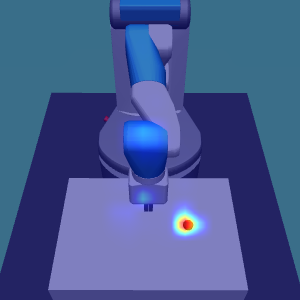
\includegraphics[width=\linewidth]{figures/chapter6/distractor_saliency_fetch_pro_off/standard_visual_std}
    \subcaption{Standard (no DR, no proprioception)}
  \end{subfigure}
  \begin{subfigure}{0.24\columnwidth}
    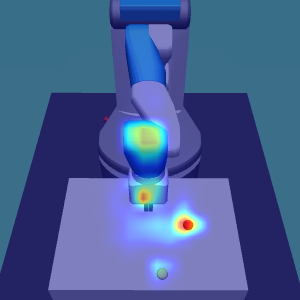
\includegraphics[width=\linewidth]{figures/chapter6/distractor_saliency_fetch_pro_off/color_visual_std}
    \subcaption{Colour (no DR, no proprioception)}
  \end{subfigure}
  \begin{subfigure}{0.24\columnwidth}
    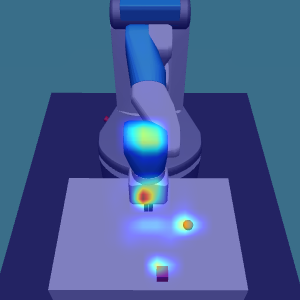
\includegraphics[width=\linewidth]{figures/chapter6/distractor_saliency_fetch_pro_off/shape_visual_std}
    \subcaption{Shape (no DR, no proprioception)}
  \end{subfigure}
  \begin{subfigure}{0.24\columnwidth}
    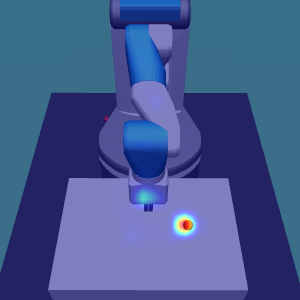
\includegraphics[width=\linewidth]{figures/chapter6/distractor_saliency_fetch_pro_on/standard_sensor_std}
    \subcaption{Standard (no DR, proprioception)}
  \end{subfigure}
  
  \begin{subfigure}{0.24\columnwidth}
    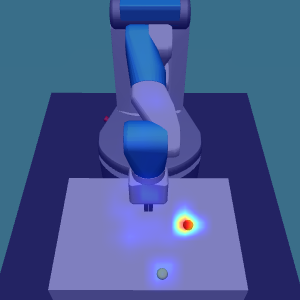
\includegraphics[width=\linewidth]{figures/chapter6/distractor_saliency_fetch_pro_on/color_sensor_std}
    \subcaption{Colour (no DR, proprioception)}
  \end{subfigure}
  \begin{subfigure}{0.24\columnwidth}
    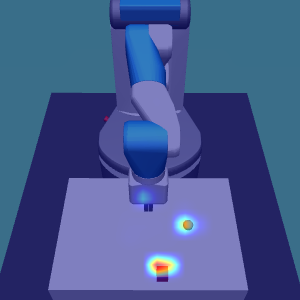
\includegraphics[width=\linewidth]{figures/chapter6/distractor_saliency_fetch_pro_on/shape_sensor_std}
    \subcaption{Shape (no DR, proprioception)}
  \end{subfigure}
  
  \begin{subfigure}{0.24\columnwidth}
    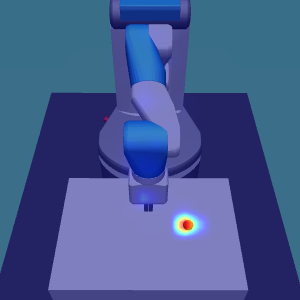
\includegraphics[width=\linewidth]{figures/chapter6/distractor_saliency_fetch_pro_off/standard_visual_random}
    \subcaption{Standard (DR, no proprioception)}
  \end{subfigure}
  \begin{subfigure}{0.24\columnwidth}
    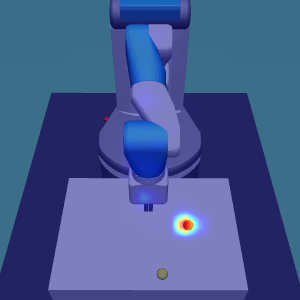
\includegraphics[width=\linewidth]{figures/chapter6/distractor_saliency_fetch_pro_off/color_visual_random}
    \subcaption{Colour (DR, no proprioception)}
  \end{subfigure}
  \begin{subfigure}{0.24\columnwidth}
    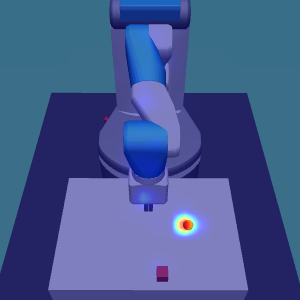
\includegraphics[width=\linewidth]{figures/chapter6/distractor_saliency_fetch_pro_off/shape_visual_random}
    \subcaption{Shape (DR, no proprioception)}
  \end{subfigure}
  \begin{subfigure}{0.24\columnwidth}
    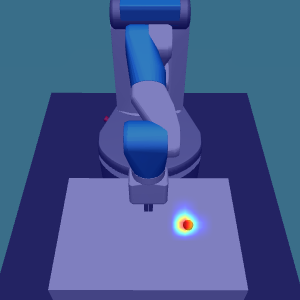
\includegraphics[width=\linewidth]{figures/chapter6/distractor_saliency_fetch_pro_on/standard_sensor_random}
    \subcaption{Standard (DR, proprioception)}
  \end{subfigure}
  
  \begin{subfigure}{0.24\columnwidth}
    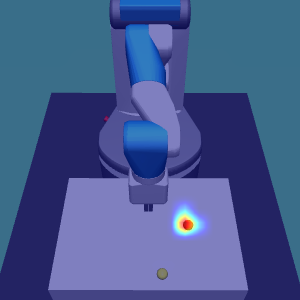
\includegraphics[width=\linewidth]{figures/chapter6/distractor_saliency_fetch_pro_on/color_sensor_random}
    \subcaption{Colour (DR, proprioception)}
  \end{subfigure}
  \begin{subfigure}{0.24\columnwidth}
    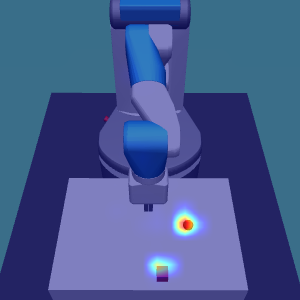
\includegraphics[width=\linewidth]{figures/chapter6/distractor_saliency_fetch_pro_on/shape_sensor_random}
    \subcaption{Shape (DR, proprioception)}
  \end{subfigure}
  \caption[Occlusion-based saliency maps of Fetch agents.]{Occlusion-based saliency maps of Fetch agents trained with (g-l) or without (a-f) DR and with (d-f, j-l) or without proprioceptive inputs (a-c, g-i) in three different test conditions (standard, colour and shape). The best Fetch model is used for each training configuration.}
  \label{fig:saliency_fetch_distractor}
\end{figure}

\begin{figure}[h!]
  \centering
  \begin{subfigure}{0.24\columnwidth}
    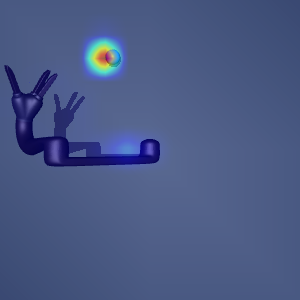
\includegraphics[width=\linewidth]{figures/chapter6/distractor_saliency_jaco_pro_off/standard_visual_std}
    \subcaption{Standard (no DR, no proprioception)}
  \end{subfigure}
  \begin{subfigure}{0.24\columnwidth}
    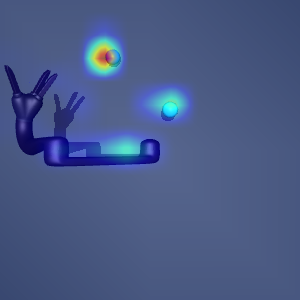
\includegraphics[width=\linewidth]{figures/chapter6/distractor_saliency_jaco_pro_off/color_visual_std}
    \subcaption{Colour (no DR, no proprioception)}
  \end{subfigure}
  \begin{subfigure}{0.24\columnwidth}
    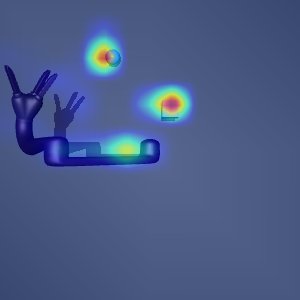
\includegraphics[width=\linewidth]{figures/chapter6/distractor_saliency_jaco_pro_off/shape_visual_std}
    \subcaption{Shape (no DR, no proprioception)}
  \end{subfigure}
  \begin{subfigure}{0.24\columnwidth}
    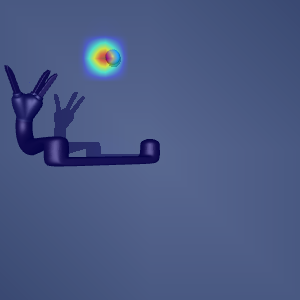
\includegraphics[width=\linewidth]{figures/chapter6/distractor_saliency_jaco_pro_on/standard_sensor_std}
    \subcaption{Standard (no DR, proprioception)}
  \end{subfigure}
  
  \begin{subfigure}{0.24\columnwidth}
    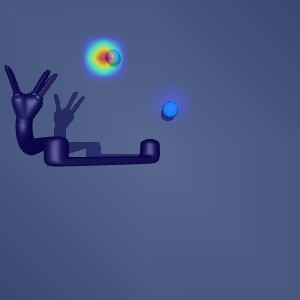
\includegraphics[width=\linewidth]{figures/chapter6/distractor_saliency_jaco_pro_on/color_sensor_std}
    \subcaption{Colour (no DR, proprioception)}
  \end{subfigure}
  \begin{subfigure}{0.24\columnwidth}
    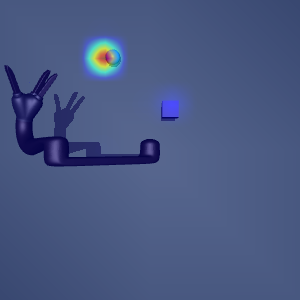
\includegraphics[width=\linewidth]{figures/chapter6/distractor_saliency_jaco_pro_on/shape_sensor_std}
    \subcaption{Shape (no DR, proprioception)}
  \end{subfigure}
  
  \begin{subfigure}{0.24\columnwidth}
    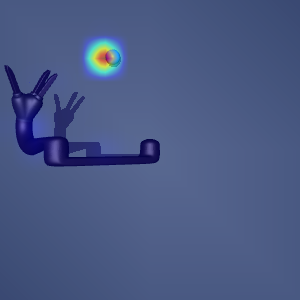
\includegraphics[width=\linewidth]{figures/chapter6/distractor_saliency_jaco_pro_off/standard_visual_random}
    \subcaption{Standard (DR, no proprioception)}
  \end{subfigure}
  \begin{subfigure}{0.24\columnwidth}
    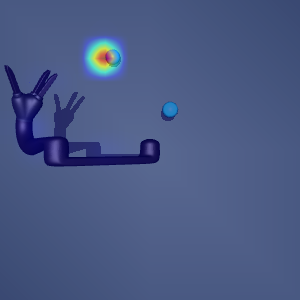
\includegraphics[width=\linewidth]{figures/chapter6/distractor_saliency_jaco_pro_off/color_visual_random}
    \subcaption{Colour (DR, no proprioception)}
  \end{subfigure}
  \begin{subfigure}{0.24\columnwidth}
    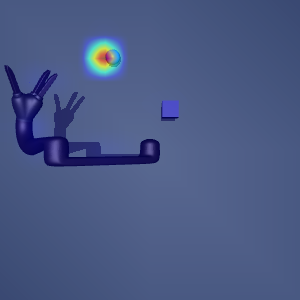
\includegraphics[width=\linewidth]{figures/chapter6/distractor_saliency_jaco_pro_off/shape_visual_random}
    \subcaption{Shape (DR, no proprioception)}
  \end{subfigure}
  \begin{subfigure}{0.24\columnwidth}
    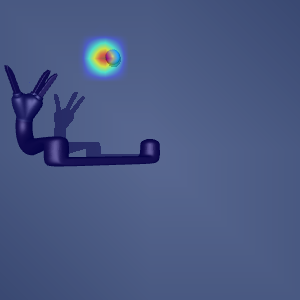
\includegraphics[width=\linewidth]{figures/chapter6/distractor_saliency_jaco_pro_on/standard_sensor_random}
    \subcaption{Standard (DR, proprioception)}
  \end{subfigure}
  
  \begin{subfigure}{0.24\columnwidth}
    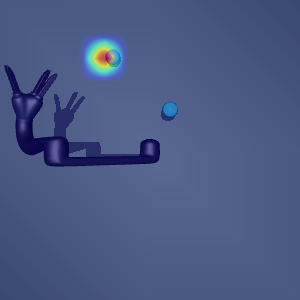
\includegraphics[width=\linewidth]{figures/chapter6/distractor_saliency_jaco_pro_on/color_sensor_random}
    \subcaption{Colour (DR, proprioception)}
  \end{subfigure}
  \begin{subfigure}{0.24\columnwidth}
    \includegraphics[width=\linewidth]{figures/chapter6/distractor_saliency_jaco_pro_on/shape_sensor_random}
    \subcaption{Shape (DR, proprioception)}
  \end{subfigure}
  \caption[[Occlusion-based saliency maps of Jaco agents.]]{Occlusion-based saliency maps of Jaco agents trained with (g-l) or without (a-f) DR and with (d-f, j-l) or without proprioceptive inputs (a-c, g-i) in three different test conditions (standard, colour and shape). The best Jaco model is used for each training configuration.}
  \label{fig:saliency_jaco_distractor}
\end{figure}

%\subsection{Statistical and Structural Weight Characterisations}
\subsection{Channel-wise Unit Ablations}

\begin{figure}[h!]
  \centering
  \begin{subfigure}{0.49\linewidth}
    \includegraphics[width=\textwidth]{figures/chapter6/unitablation/conv1_ablations}
    \caption{Standard test condition (Layer 1)}
  \end{subfigure}
  \begin{subfigure}{0.49\linewidth}
    \includegraphics[width=\textwidth]{figures/chapter6/unitablation/conv1_ablations_noisy}
    \caption{Noise test condition (Layer 1)}
  \end{subfigure}

  \begin{subfigure}{0.49\linewidth}
    \includegraphics[width=\textwidth]{figures/chapter6/unitablation/conv2_ablations}
    \caption{Standard test condition (Layer 2)}
  \end{subfigure}
  \begin{subfigure}{0.49\linewidth}
    \includegraphics[width=\textwidth]{figures/chapter6/unitablation/conv2_ablations_noisy}
    \caption{Noise test condition (Layer 2)}
  \end{subfigure}
  \caption[Test performance of unit ablation tests of the best models under 8 training configurations in standard and noise conditions.]{The performance of unit ablation tests of the trained Fetch and Jaco agents under 8 different training configurations in standard and visual noise conditions. Each point represents one unit in layer 1 (a, b) or layer 2 (c, d). The vertical bars indicate baseline performance in the test environment. The training settings correspond to the Fetch (F) and Jaco (J) robots, whether additional proprioceptive inputs are available (Prop), and if DR is activated. The best model is used for each training configuration. To be noticed that the Jaco agent trained with DR but without proprioceptive inputs has a lower baseline performance on the standard visuals than the other models (Table \ref{tbl:tests}).}
  \label{fig:unit_ablations}
\end{figure}
We use unit ablations to provide white box and quantitative analysis. We first select the best agent from each of 8 training configurations across five different seeds as our test models. Subsequently, for each test model, we mask one of the output channels to zero in the first or second convolutional layers. Then, the modified model is evaluated on both standard and noise conditions (80 fixed positions for Fetch agents and 250 fixed positions for Jaco agents). Finally, we repeat the above process until all output channels have been tested. The results of the unit ablation tests are illustrated in Figure~\ref{fig:unit_ablations}.

From Figure~\ref{fig:unit_ablations}, we observe that the impact of unit ablation on the Fetch agents is small. However, the effect on the Jaco agents is relatively large, as the performance of the Jaco agents varies significantly. This is probably because of the increased complexity of the Jaco task (e.g., control scheme), which requires more powerful channels to extract relevant information to train the agents.

% We further find that the unit ablations can improve the performance in the noise condition, even for the DR agents. \td{This may}
Furthermore, in the first convolutional layer (see Figure~\ref{fig:unit_ablations}a,b), there exist several extremely critical channels/units that can substantially affect the performance of the agent. However, there are no such channels in the second convolutional layer (see Figure~\ref{fig:unit_ablations}c,d).

Next, we find that the variability in the noisy environment (see Figure~\ref{fig:unit_ablations}b,d) is greater. Intriguingly, ablations can improve performance beyond the baseline results, even for agents trained with DR---perhaps indicating a sensitivity to high-frequency noise. Although a detailed discussion is beyond the scope of this work, we note that research on corruption and adversarial robustness in supervised learning settings could provide further insights on properties such as these~\cite{gilmer2019adversarial, hendrycks2019benchmarking}.

\subsection{Layer Re-initialisation}
Next, we move to the layer re-initialisation test, where we evaluate models' robustness to the layer re-initialisation and the change of the parameters in $\ell_{\infty}$ and $\ell_{2}$ norm. The related plots of Fetch and Jaco agents are in Figure~\ref{fig:fetch_robustness} and Figure~\ref{fig:jaco_robustness}, respectively. Generally, after a period of training, the LSTM layer and policy layer are more robust to be re-initialised with the initial weights. For the agents trained with DR, they show less robustness to re-initialisation from the early to middle stages of training, which indicates that the agents trained with DR require longer periods to learn useful representations from tasks.

Another interesting finding is that when the proprioceptive inputs are available, the first fully connected layer (fc1) of the agents needs more extended periods for training. This is probably because the fc1 layer has to learn a sophisticated combination between the visual inputs and proprioceptive inputs. This is especially the case for the Jaco agent trained with DR, which can use only proprioceptive inputs for pose estimation: it requires an even longer time to train the fc1 layer than other agents (see Figure~\ref{fig:jaco_robustness}j).

Finally, in almost all cases, the LSTM layer is robust to be re-initialised with the initial weights. One possible explanation is, the LSTM layer learns a trivial mapping within the network. Further experiments to verify this assumption are provided in the following subsection.
%Therefore, we suppose that the LSTM layer is redundant in the network structure for these tasks. 

\begin{figure}[h!]
  \centering
  \begin{subfigure}{0.32\textwidth}
    \includegraphics[width=\textwidth]{figures/chapter6/robustness/fetch/visual_std/error}
    \caption{Robustness (no DR, no proprioception)}
  \end{subfigure}
  \begin{subfigure}{0.32\textwidth}
    \includegraphics[width=\textwidth]{figures/chapter6/robustness/fetch/visual_std/inf_dist}
    \caption{$\ell_\infty$-norm (no DR, no proprioception)}
  \end{subfigure}
  \begin{subfigure}{0.32\textwidth}
    \includegraphics[width=\textwidth]{figures/chapter6/robustness/fetch/visual_std/l2_dist}
    \caption{$\ell_2$-norm (no DR, no proprioception)}
  \end{subfigure}
  \begin{subfigure}{0.32\textwidth}
    \includegraphics[width=\textwidth]{figures/chapter6/robustness/fetch/sensor_std/error}
    \caption{Robustness (no DR, proprioception)}
  \end{subfigure}
  \begin{subfigure}{0.32\textwidth}
    \includegraphics[width=\textwidth]{figures/chapter6/robustness/fetch/sensor_std/inf_dist}
    \caption{$\ell_\infty$-norm (no DR, proprioception)}
  \end{subfigure}
  \begin{subfigure}{0.32\textwidth}
    \includegraphics[width=\textwidth]{figures/chapter6/robustness/fetch/sensor_std/l2_dist}
    \caption{$\ell_2$-norm (no DR, proprioception)}
  \end{subfigure}
  \begin{subfigure}{0.32\textwidth}
    \includegraphics[width=\textwidth]{figures/chapter6/robustness/fetch/visual_random/error}
    \caption{Robustness (DR, no proprioception)}
  \end{subfigure}
  \begin{subfigure}{0.32\textwidth}
    \includegraphics[width=\textwidth]{figures/chapter6/robustness/fetch/visual_random/inf_dist}
    \caption{$\ell_\infty$-norm (DR, no proprioception)}
  \end{subfigure}
  \begin{subfigure}{0.32\textwidth}
    \includegraphics[width=\textwidth]{figures/chapter6/robustness/fetch/visual_random/l2_dist}
    \caption{$\ell_2$-norm (DR, no proprioception)}
  \end{subfigure}
  \begin{subfigure}{0.32\textwidth}
    \includegraphics[width=\textwidth]{figures/chapter6/robustness/fetch/sensor_random/error}
    \caption{Robustness (DR, proprioception)}
  \end{subfigure}
  \begin{subfigure}{0.32\textwidth}
    \includegraphics[width=\textwidth]{figures/chapter6/robustness/fetch/sensor_random/inf_dist}
    \caption{$\ell_\infty$-norm (DR, proprioception)}
  \end{subfigure}
  \begin{subfigure}{0.32\textwidth}
    \includegraphics[width=\textwidth]{figures/chapter6/robustness/fetch/sensor_random/l2_dist}
    \caption{$\ell_2$-norm (DR, proprioception)}
  \end{subfigure}
  \caption[Test performance of re-initialisation robustness and change of parameters of Fetch agents.]{Performance of re-initialisation robustness (0 for 100$\%$ success rate, and 1 for 0$\%$ success rate), and change of parameters in $\ell_\infty$- and $\ell_2$-norm of Fetch agents. The best Fetch model is selected for each training configuration.}
  \label{fig:fetch_robustness}
\end{figure}
%\vspace{-15mm}
\begin{figure}[h!]
  \centering
  \begin{subfigure}{0.32\textwidth}
    \includegraphics[width=\textwidth]{figures/chapter6/robustness/jaco/visual_std/error}
    \caption{Robustness (no DR, no proprioception)}
  \end{subfigure}
  \begin{subfigure}{0.32\textwidth}
    \includegraphics[width=\textwidth]{figures/chapter6/robustness/jaco/visual_std/inf_dist}
    \caption{$\ell_\infty$-norm (no DR, no proprioception)}
  \end{subfigure}
  \begin{subfigure}{0.32\textwidth}
    \includegraphics[width=\textwidth]{figures/chapter6/robustness/jaco/visual_std/l2_dist}
    \caption{$\ell_2$-norm (no DR, no proprioception)}
  \end{subfigure}
  \begin{subfigure}{0.32\textwidth}
    \includegraphics[width=\textwidth]{figures/chapter6/robustness/jaco/sensor_std/error}
    \caption{Robustness (no DR, proprioception)}
  \end{subfigure}
  \begin{subfigure}{0.32\textwidth}
    \includegraphics[width=\textwidth]{figures/chapter6/robustness/jaco/sensor_std/inf_dist}
    \caption{$\ell_\infty$-norm (no DR, proprioception)}
  \end{subfigure}
  \begin{subfigure}{0.32\textwidth}
    \includegraphics[width=\textwidth]{figures/chapter6/robustness/jaco/sensor_std/l2_dist}
    \caption{$\ell_2$-norm (no DR, proprioception)}
  \end{subfigure}
  \begin{subfigure}{0.32\textwidth}
    \includegraphics[width=\textwidth]{figures/chapter6/robustness/jaco/visual_random/error}
    \caption{Robustness (DR, no proprioception)}
  \end{subfigure}
  \begin{subfigure}{0.32\textwidth}
    \includegraphics[width=\textwidth]{figures/chapter6/robustness/jaco/visual_random/inf_dist}
    \caption{$\ell_\infty$-norm (DR, no proprioception)}
  \end{subfigure}
  \begin{subfigure}{0.32\textwidth}
    \includegraphics[width=\textwidth]{figures/chapter6/robustness/jaco/visual_random/l2_dist}
    \caption{$\ell_2$-norm (DR, no proprioception)}
  \end{subfigure}
  \begin{subfigure}{0.32\textwidth}
    \includegraphics[width=\textwidth]{figures/chapter6/robustness/jaco/sensor_random/error}
    \caption{Robustness (DR, proprioception)}
  \end{subfigure}
  \begin{subfigure}{0.32\textwidth}
    \includegraphics[width=\textwidth]{figures/chapter6/robustness/jaco/sensor_random/inf_dist}
    \caption{$\ell_\infty$-norm (DR, proprioception)}
  \end{subfigure}
  \begin{subfigure}{0.32\textwidth}
    \includegraphics[width=\textwidth]{figures/chapter6/robustness/jaco/sensor_random/l2_dist}
    \caption{$\ell_2$-norm (DR, proprioception)}
  \end{subfigure}
  \caption[Test performance of re-initialisation robustness and change of parameters of Jaco agents.]{Performance of re-initialisation robustness (0 for 100$\%$ success rate, and 1 for 0$\%$ success rate), and change of parameters in $\ell_\infty$- and $\ell_2$-norm of Jaco agents. The best Fetch model is selected for each training configuration.}
  %Note that the final failure rate of the best Jaco agent trained with DR and without proprioception on the standard environment is around 20\%. The re-initialisation robustness plot for this condition (g) indicates that all layers are necessary and that training continues to improve performance in the epochs depicted and beyond.
  \label{fig:jaco_robustness}
\end{figure}

\subsection{Recurrent Ablation}
\label{sec:detail_reucrrent_ablation}
We then evaluate the effectiveness of the LSTM layer for the training. In this case, the \textit{hidden} and \textit{cell} states are set to constant values for the evaluation. Instead of simply setting the hidden and cell states to zero -- as this may not represent the normal value in the rollouts, at each timestep -- we set the hidden and cell states to empirical average values which are calculated over the generated values of the models in testing (80 episodes for the Fetch agents and 250 episodes for the Jaco agents). From Table~\ref{tbl:hidden_ablation}, the LSTM layer with constant values only has a minor influence on agents trained without DR, while it has a significant influence on the agents trained with DR. This suggests that the LSTM layer is functional when DR is activated during training, otherwise it only learns a trivial mapping within the network. One possible explanation is that when DR is not activated during training, the textures and colours of the background in the environment remain unchanged, the agent only needs to learn the policy that keeps moving towards the target object in each frame. Therefore, in this case, the sequence information is not that crucial, and the LSTM layer does not play an important role. When DR is activated during training, the textures and colours of the background in the environment change in every frame. When the textures or colours of the background are similar to the target object, the agent needs to use the sequence information to remember the location of the target object in the previous frames to distinguish the target from irrelevant information and complete the task. Therefore, when DR is activated during training, the LSTM layer needs to capture the location of the target object in previous frames. In terms of the strategies \emph{learned} by the agents (Figure \ref{fig:strategies}), memory is sufficient for the agents trained without DR, but necessary for the agents trained with DR.

\begin{table}[h!]
  \centering
  \begin{tabular}{c|cc|cc}
    \toprule
    Robot & DR & Prop. & Standard & Constant Hidden\\
    \midrule
    Fetch & {\xmark} & {\xmark} & 1.000$\pm 0.000$ & 0.988$\pm 0.016$\\
    Fetch & {\xmark} & {\cmark} & 1.000$\pm 0.000$ & 0.990$\pm 0.012$\\
    Fetch & {\cmark} & {\xmark} & 0.983$\pm 0.004$ & 0.658$\pm 0.106$\\
    Fetch & {\cmark} & {\cmark} & 0.997$\pm 0.002$ & 0.838$\pm 0.051$\\
    \hline
    Jaco  & {\xmark} & {\xmark} & 0.995$\pm 0.003$ & 0.919$\pm 0.032$\\
    Jaco  & {\xmark} & {\cmark} & 0.995$\pm 0.001$ & 0.943$\pm 0.022$\\
    Jaco  & {\cmark} & {\xmark} & 0.650$\pm 0.056$ & 0.422$\pm 0.083$\\
    Jaco  & {\cmark} & {\cmark} & 0.991$\pm 0.004$ & 0.746$\pm 0.060$\\
    \bottomrule
  \end{tabular}
  \caption[Test performance of recurrent ablations of all models.]{Performance of recurrent ablations of all models with standard operation and constant (empirical average) hidden states. Checkmarks and crosses indicate activate/deactivate DR and proprioceptive inputs (Prop.), respectively. Mean $\pm$ standard error are calculated over all models (seeds) and test target locations.}
  \label{tbl:hidden_ablation}
\end{table}
% discussion
\section{Discussion}
This chapter aims to analyse and understand what strategies and representations the agents have learned in a simulated robot manipulation task, especially with domain randomisation (DR). In this experiment, we construct 8 different training configurations, which cover different morphologies and control schemes of the robot arm (Fetch and Jaco robot arms), different modalities of inputs (visual inputs or visual + proprioceptive inputs), and using or not using DR. We also setup 8 different test conditions to evaluate the agents' robustness to local and global visual changes and the ability of visual pose estimation. Finally, various interpretability techniques are adopted to provide both quantitative and qualitative analysis of the agents.

From the results, the agent trained with DR shows better generalisation ability to local visual changes, such as distractors with different colours and shapes. While agents trained with DR also present a degree of robustness to global visual changes, such as illumination (direction and intensity), RGB camera translation, additive noise, and reflective surfaces, they still show significant performance degradation in several scenarios. The above failure cases can remind us to consider more factors in the design of the algorithms/settings to perform domain randomisation, where we only focus on visual DR in this chapter (e.g., texture, colours, and noise). From saliency maps, the agents trained without DR show more highlighted regions over the distractors, and the agents trained with DR focus more attention on the task-related objects (e.g., robot arm and target ball). 

In unit ablations, due to the task complexity and the control scheme of the Jaco environment, the Jaco agents require more channels for learning the representations to solve the task (see  Figure~\ref{fig:unit_ablations}). In layer re-initialisation, DR leads to distinguishable changes in $\ell_{\infty}$-norm of parameters in the convolutional layers and therefore acquires more robust features. Figure~\ref{fig:jaco_robustness} also shows that, when the proprioceptive inputs are available, the fc1 layer of the Jaco agent trained with DR requires longer periods for training,  because it needs to learn a better representation from proprioceptive inputs for pose estimation. This trend is also in line with the results in the test condition of invisible robot arms, where this agent can still perform the task without the rendered robot arm. In this case, the agent only utilises proprioceptive inputs to infer the location of the robot arm. In the test of recurrent ablations, the LSTM layer is only necessary when DR is activated.

Finally, some recommendations can also be provided as a result of the experiments performed in this chapter.
%are also provided to those who intend to investigate DRL agents.
\begin{itemize}
\item[1)] Do not assume that results generalise. While the Jaco agent trained with DR and without proprioception obeys some trends, it remains an outlier in many other aspects.
\item[2)] Do not expect to obtain distinct trends in the results of an interpretability method in response to apparently clear differences between two environments. While some methods, such as the saliency map, uncovered clear trends, others, such as unit ablations, did not. If possible, use a range of interpretability methods. Uncertainty about results from one method may be resolved by results from another method.
%This does not mean that unit ablations are generally useless---one can imagine that if several units were highly important without DR and no units are individually important with DR, we would have found a significant trend using this method.
\item[3)] Finally, use interpretability methods before making claims about the strategies used by agents. While one may assume that an agent that performs well at a task on average is using an intelligent strategy, in all likelihood, it may be using heuristics that fail to generalise \cite{ruderman2019uncovering}.
\end{itemize}

\label{ch6:discussion}